\documentclass[10pt]{article}
\usepackage[utf8]{inputenc}\usepackage[T1]{fontenc}\usepackage[spanish]{babel}
\usepackage{geometry,graphicx,booktabs,hyperref}
\geometry{margin=1.7cm}\graphicspath{{../../../outputs/parte_2/12_atlas/}}
\title{Atlas de clusters espaciales — Parte 2}\author{Proyecto Cuenca del Alto Atoyac}\date{Septiembre de 2026}
\begin{document}\maketitle
\noindent Las fichas utilizan la solución espacial principal fija. La composición económica se calcula posteriormente. \texttt{RUIDO\_DISPERSO} es un grupo comparativo, no un cluster equivalente.\tableofcontents\clearpage

\section*{Actividad dispersa}
\addcontentsline{toc}{section}{Actividad dispersa}
\begin{center}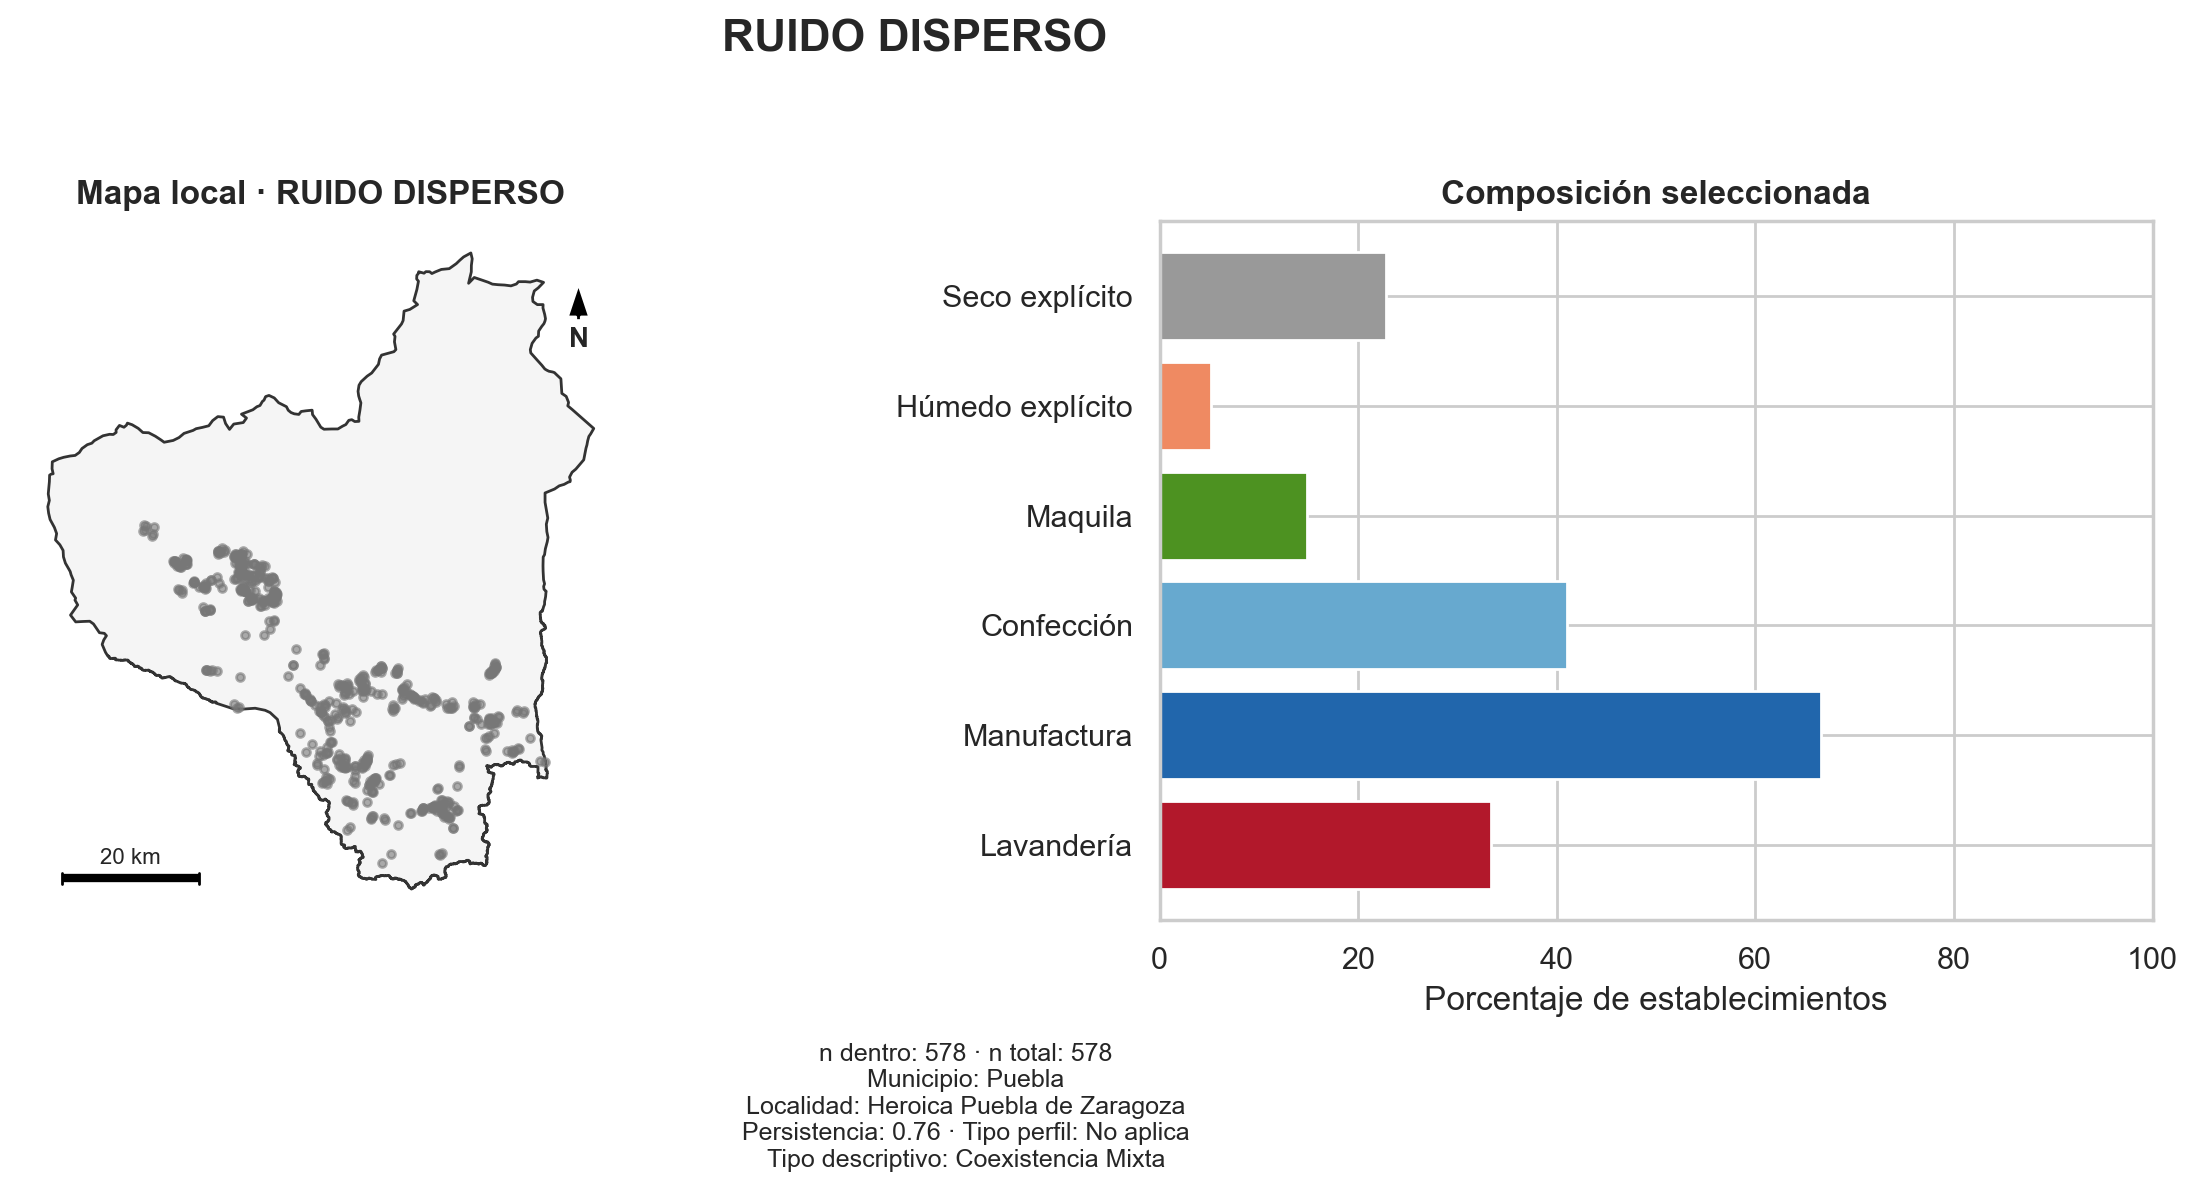
\includegraphics[width=\textwidth]{ruido_disperso.png}\end{center}
\begin{tabular}{p{0.31\textwidth}p{0.62\textwidth}}
\toprule
Establecimientos & 578 dentro; 0 fuera; 578 total\\
Área convexa & No aplica\\
Persistencia & 0.759\\
Municipio/localidad dominante & Puebla / Heroica Puebla de Zaragoza\\
Lavandería / manufactura & 33.4\% / 66.6\%\\
Confección / maquila & 41.0\% / 14.9\%\\
Húmedo / seco explícito & 5.2\% / 22.8\%\\
Tipología de perfil & No aplica\\
Rasgos distintivos & proceso\_seco\_explicito (lift 1.42)\\
Advertencia & Grupo comparativo; no es un cluster territorial.\\
\bottomrule
\end{tabular}
\clearpage

\section*{Cluster 004}
\addcontentsline{toc}{section}{Cluster 004}
\begin{center}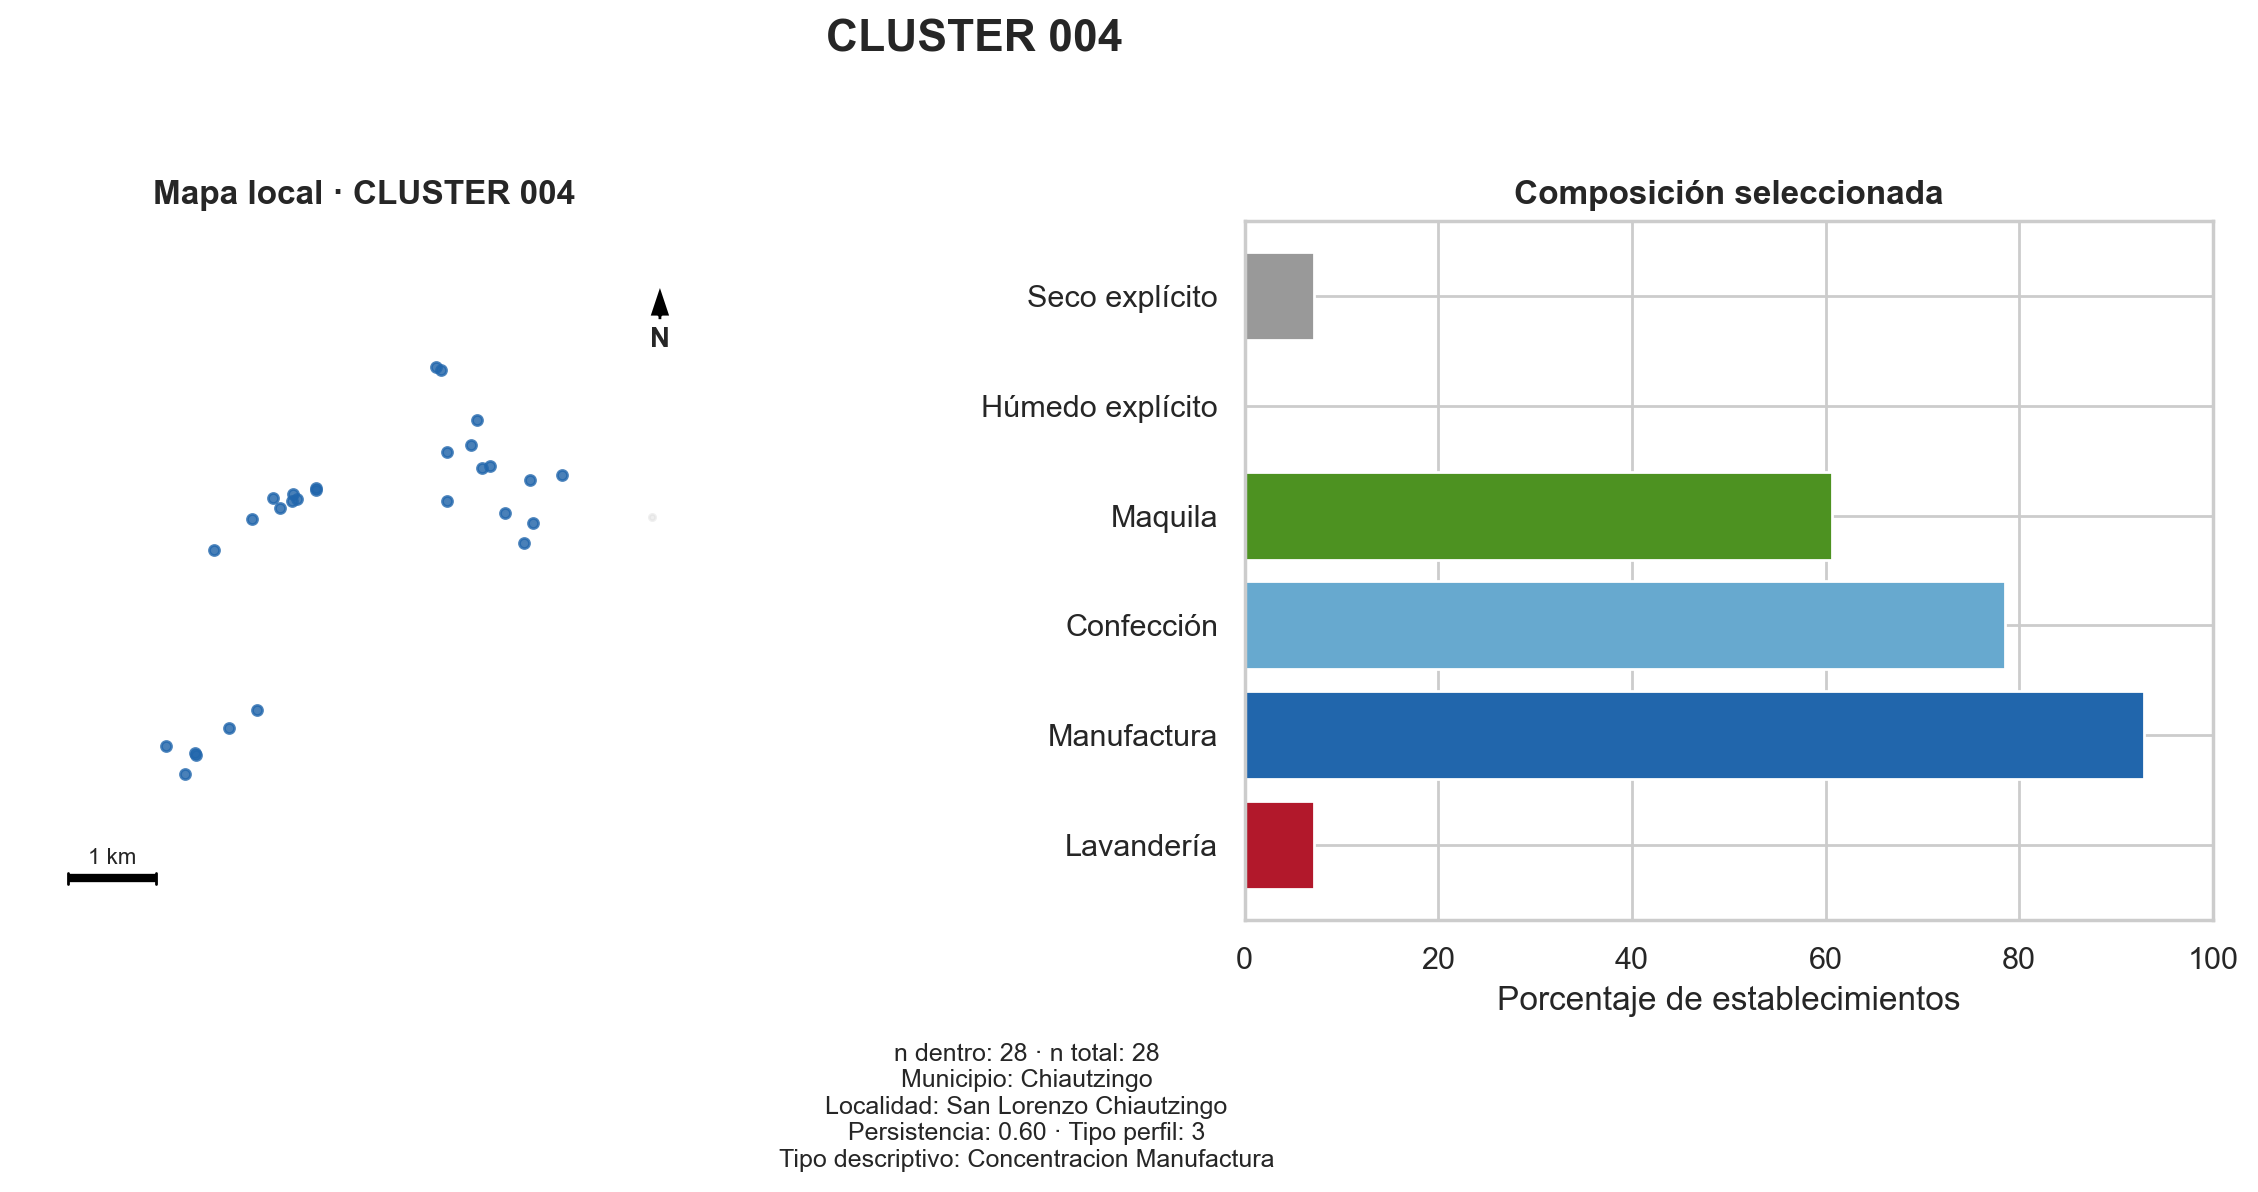
\includegraphics[width=\textwidth]{cluster_004.png}\end{center}
\begin{tabular}{p{0.31\textwidth}p{0.62\textwidth}}
\toprule
Establecimientos & 28 dentro; 0 fuera; 28 total\\
Área convexa & 9.27 km$^2$\\
Persistencia & 0.600\\
Municipio/localidad dominante & Chiautzingo / San Lorenzo Chiautzingo\\
Lavandería / manufactura & 7.1\% / 92.9\%\\
Confección / maquila & 78.6\% / 60.7\%\\
Húmedo / seco explícito & 0.0\% / 7.1\%\\
Tipología de perfil & 3.0\\
Rasgos distintivos & maquila (lift 4.13) | actividad\_confeccion (lift 2.02) | scian\_textil (lift 1.54)\\
Advertencia & Perfil descriptivo multilabel; no prueba relaciones productivas ni ambientales.\\
\bottomrule
\end{tabular}
\clearpage

\section*{Cluster 005}
\addcontentsline{toc}{section}{Cluster 005}
\begin{center}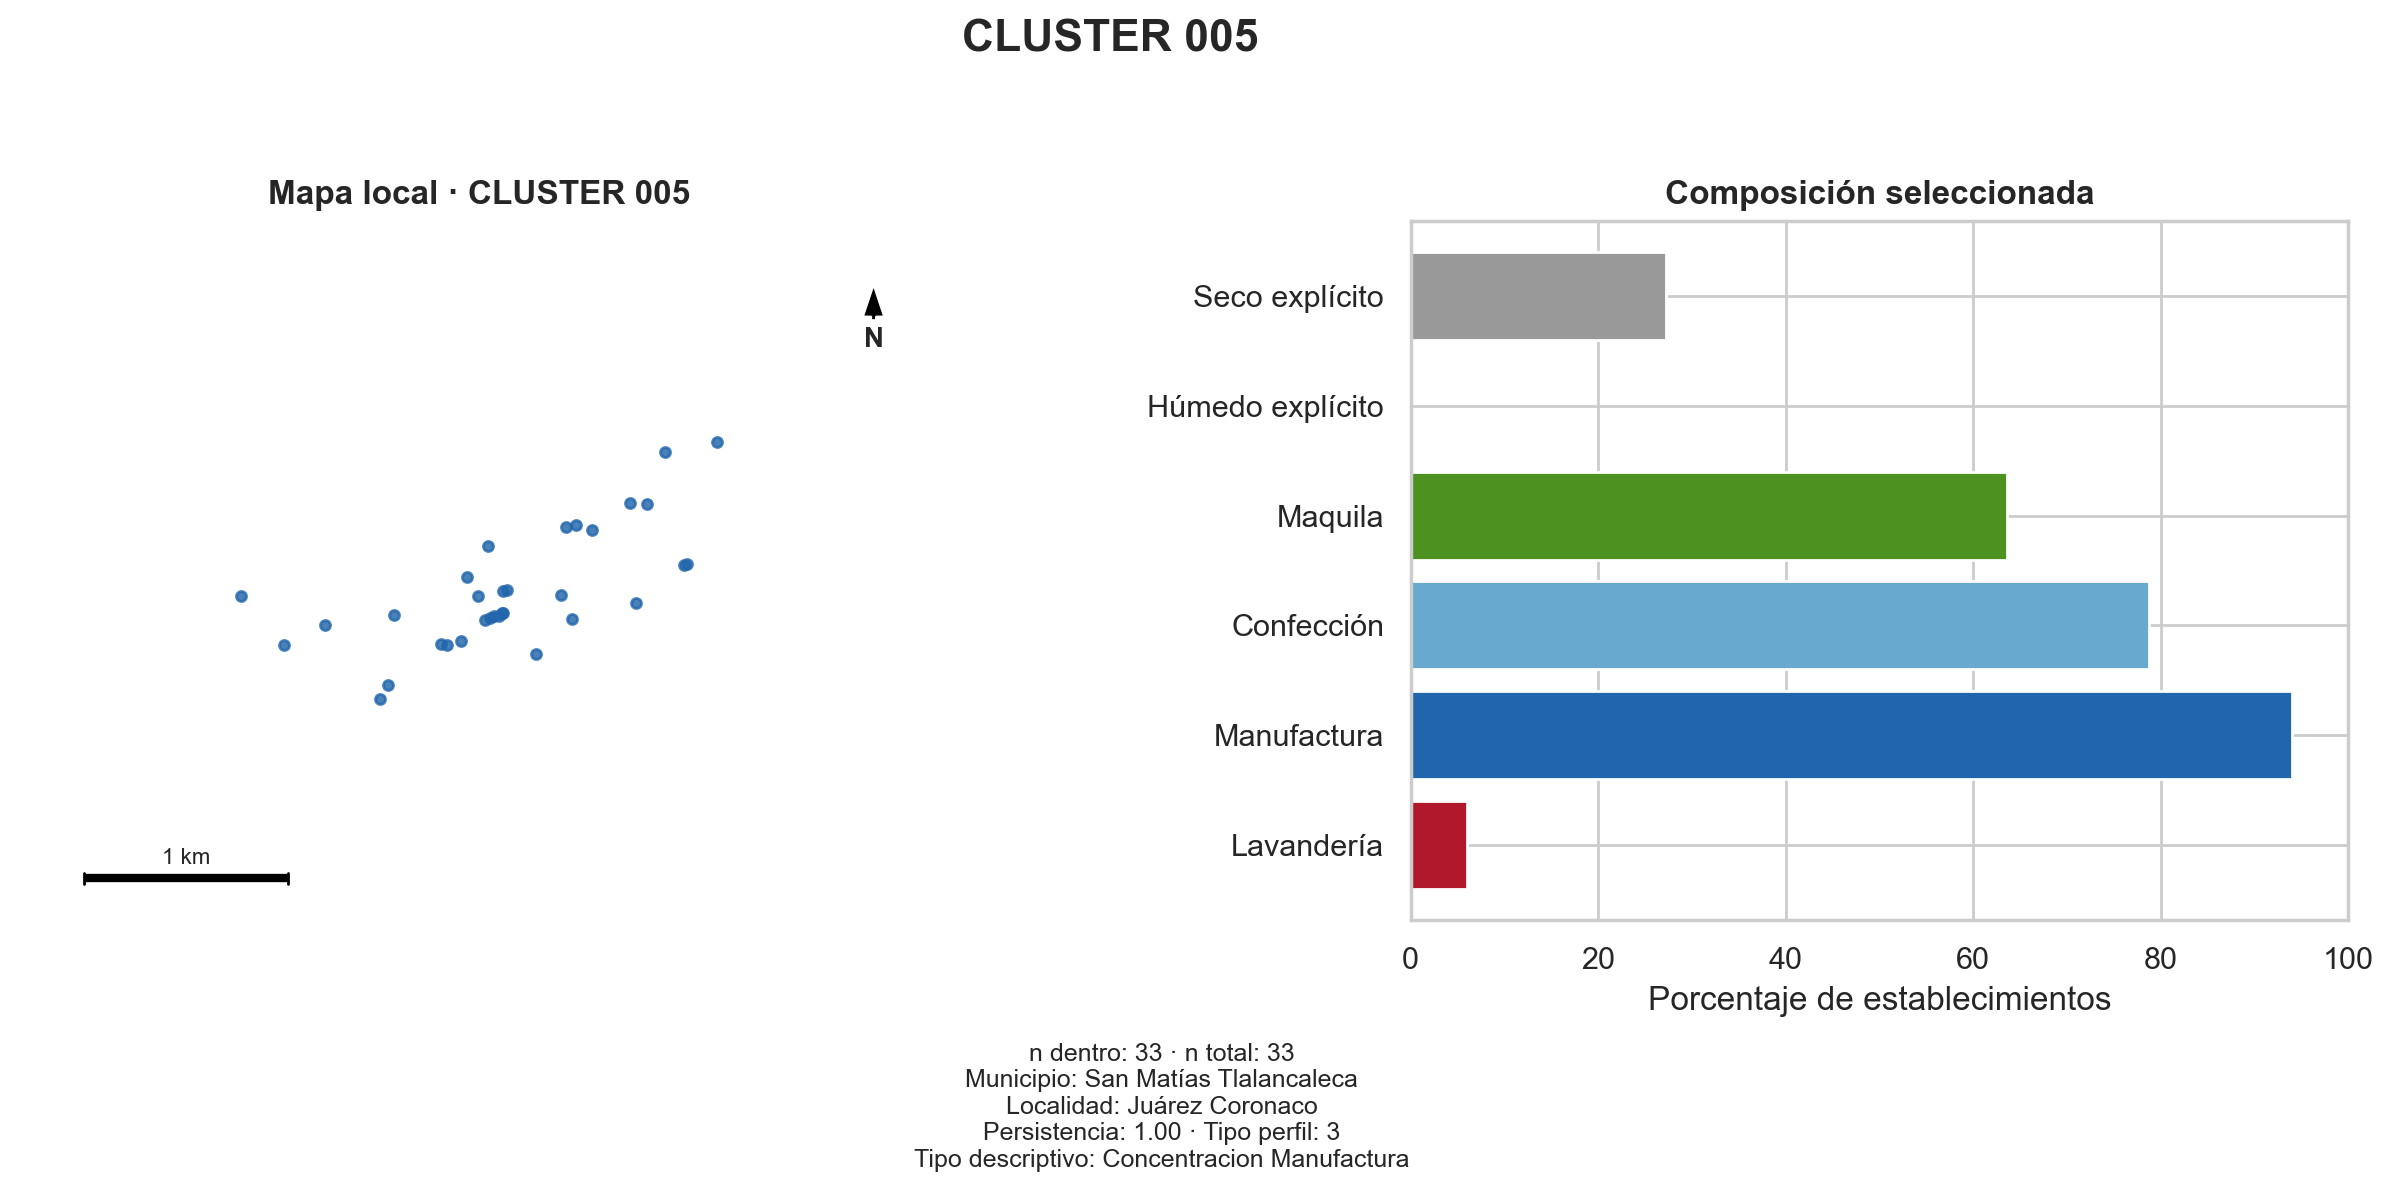
\includegraphics[width=\textwidth]{cluster_005.png}\end{center}
\begin{tabular}{p{0.31\textwidth}p{0.62\textwidth}}
\toprule
Establecimientos & 33 dentro; 0 fuera; 33 total\\
Área convexa & 1.42 km$^2$\\
Persistencia & 1.000\\
Municipio/localidad dominante & San Matías Tlalancaleca / Juárez Coronaco\\
Lavandería / manufactura & 6.1\% / 93.9\%\\
Confección / maquila & 78.8\% / 63.6\%\\
Húmedo / seco explícito & 0.0\% / 27.3\%\\
Tipología de perfil & 3.0\\
Rasgos distintivos & maquila (lift 4.33) | actividad\_confeccion (lift 2.02) | scian\_textil (lift 1.55)\\
Advertencia & Perfil descriptivo multilabel; no prueba relaciones productivas ni ambientales.\\
\bottomrule
\end{tabular}
\clearpage

\section*{Cluster 006}
\addcontentsline{toc}{section}{Cluster 006}
\begin{center}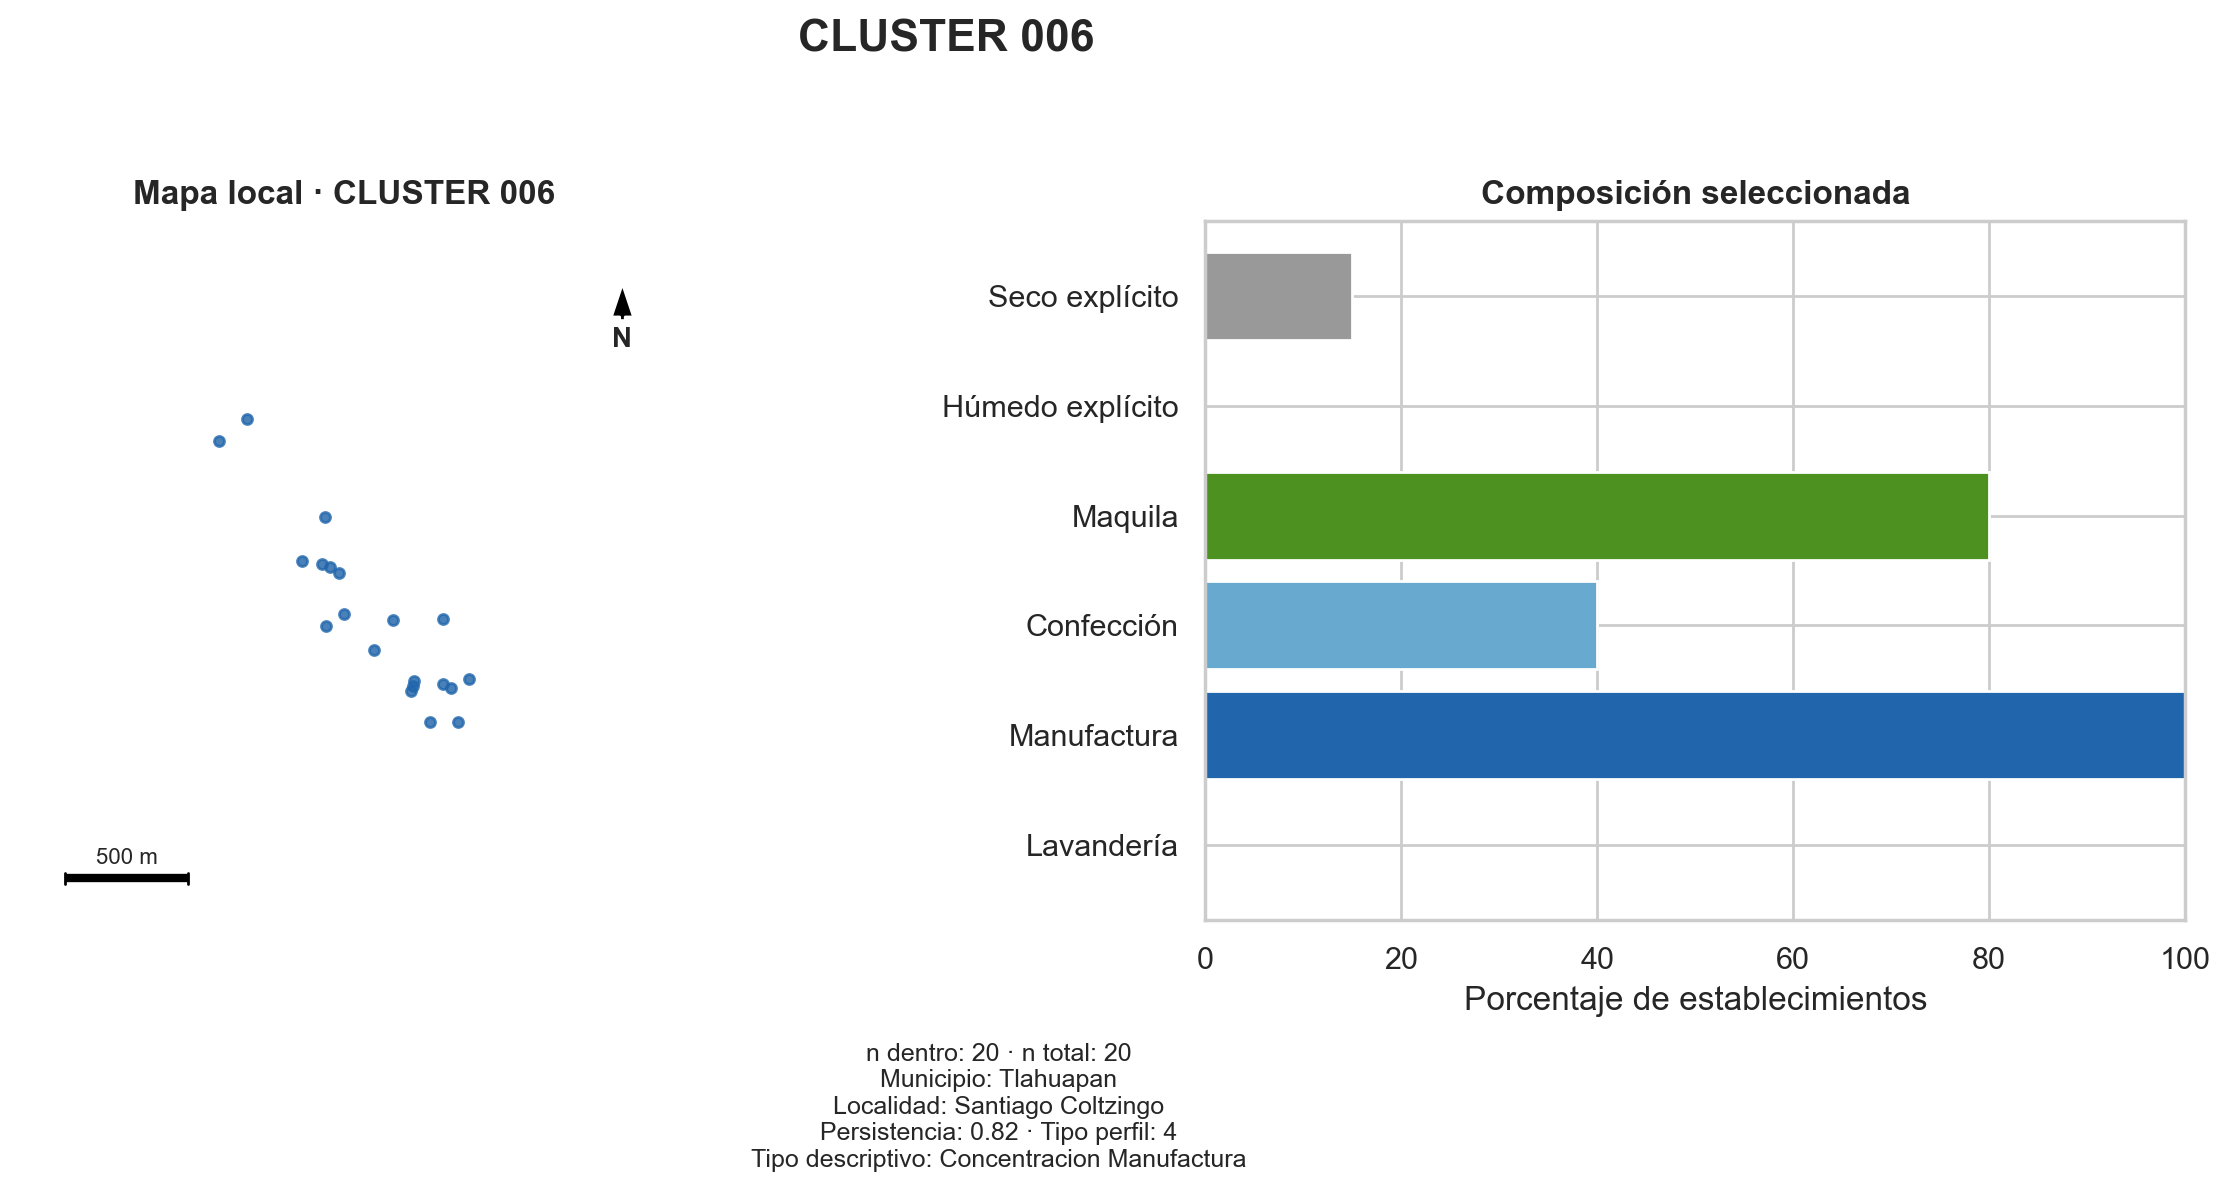
\includegraphics[width=\textwidth]{cluster_006.png}\end{center}
\begin{tabular}{p{0.31\textwidth}p{0.62\textwidth}}
\toprule
Establecimientos & 20 dentro; 0 fuera; 20 total\\
Área convexa & 0.40 km$^2$\\
Persistencia & 0.820\\
Municipio/localidad dominante & Tlahuapan / Santiago Coltzingo\\
Lavandería / manufactura & 0.0\% / 100.0\%\\
Confección / maquila & 40.0\% / 80.0\%\\
Húmedo / seco explícito & 0.0\% / 15.0\%\\
Tipología de perfil & 4.0\\
Rasgos distintivos & maquila (lift 5.45) | scian\_textil (lift 1.65)\\
Advertencia & Perfil descriptivo multilabel; no prueba relaciones productivas ni ambientales.\\
\bottomrule
\end{tabular}
\clearpage

\section*{Cluster 007}
\addcontentsline{toc}{section}{Cluster 007}
\begin{center}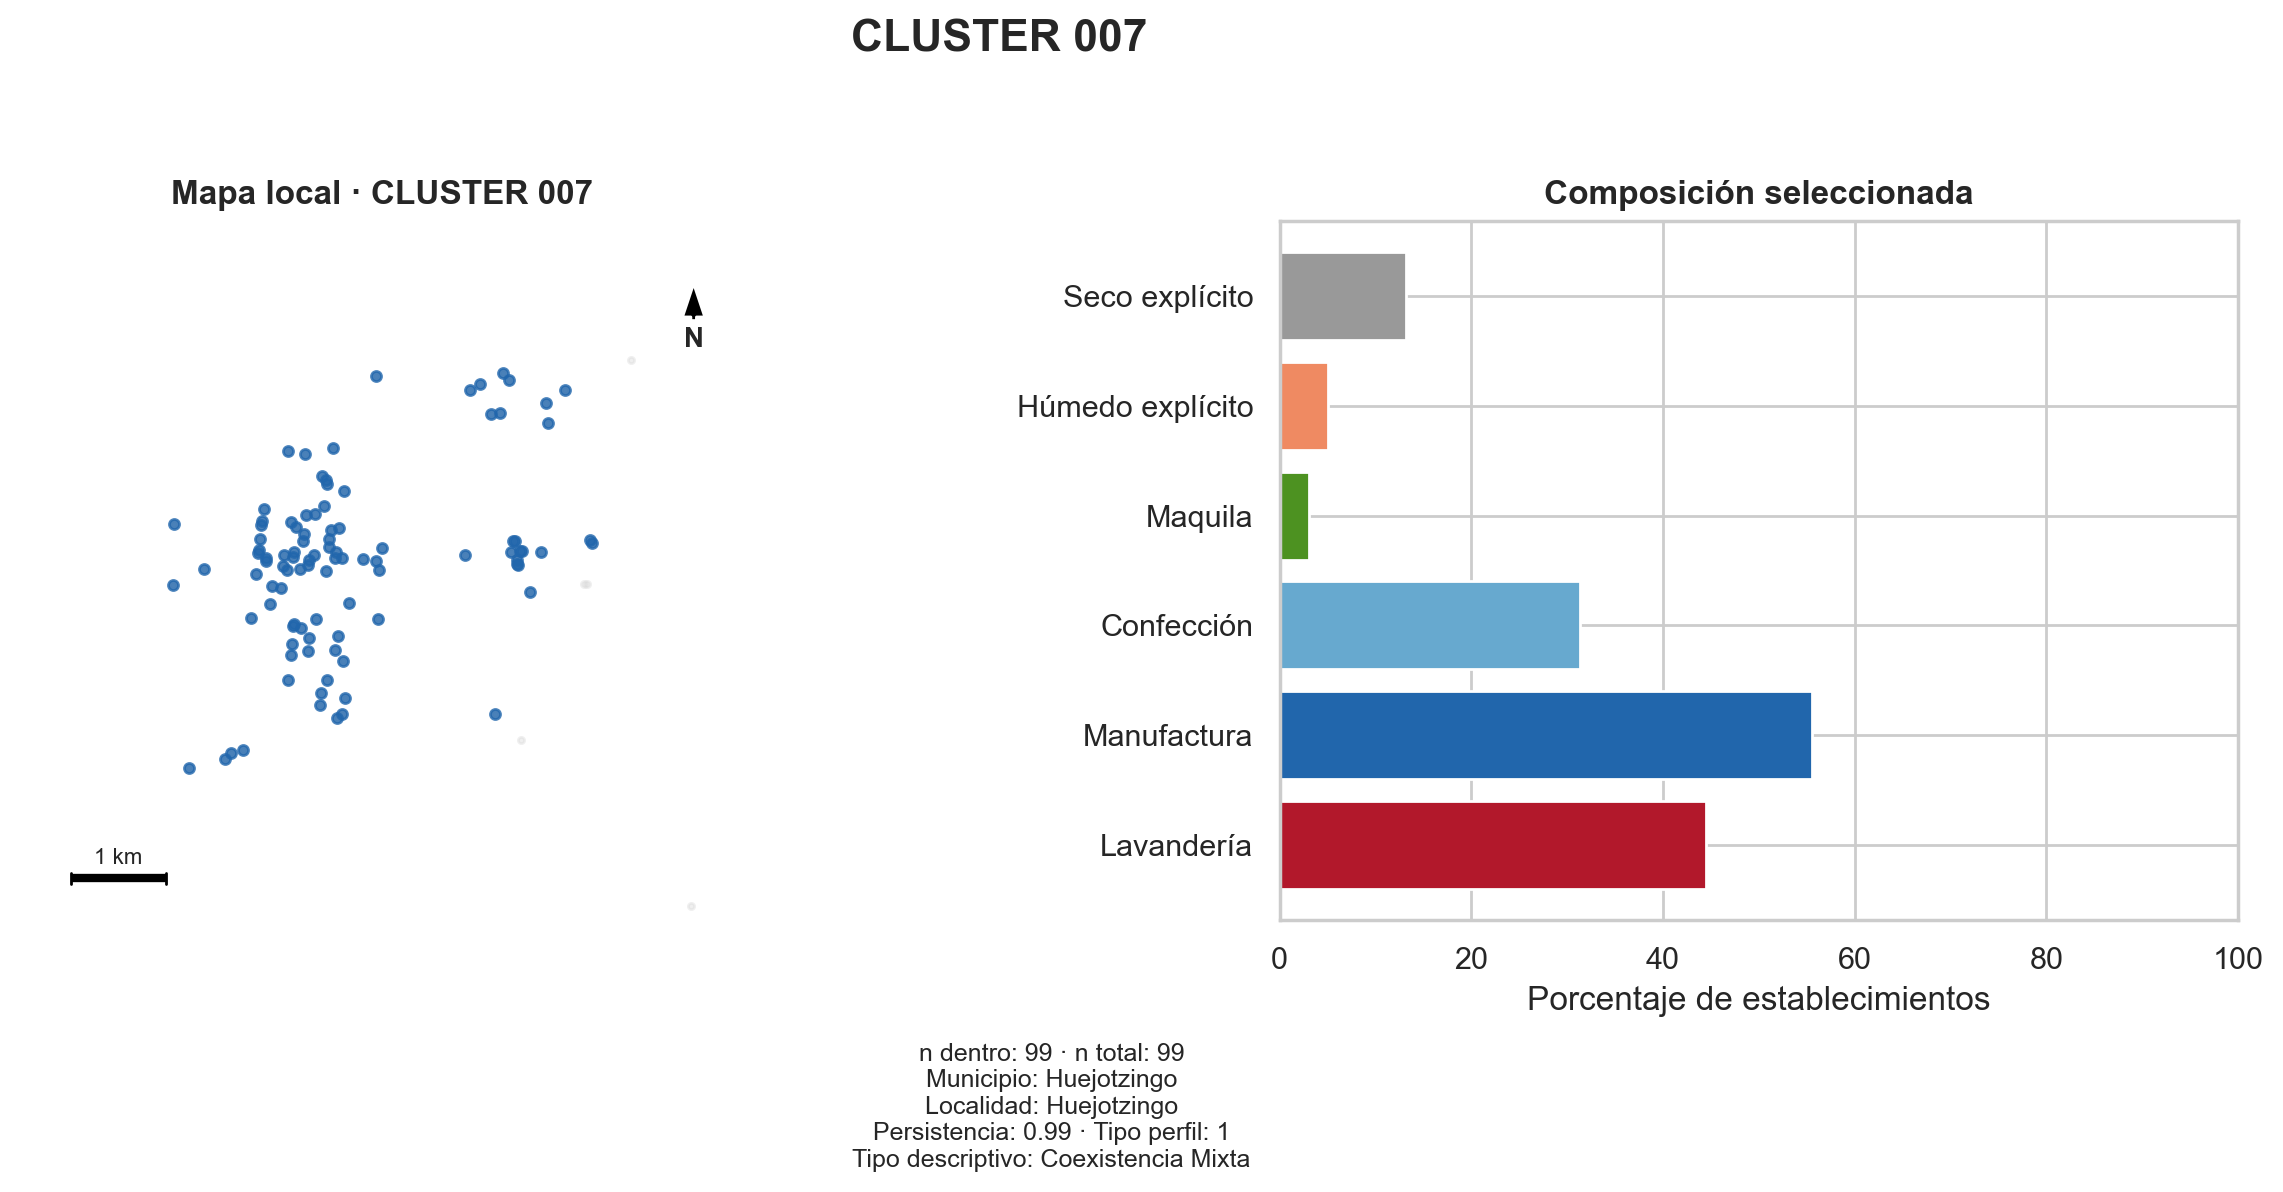
\includegraphics[width=\textwidth]{cluster_007.png}\end{center}
\begin{tabular}{p{0.31\textwidth}p{0.62\textwidth}}
\toprule
Establecimientos & 99 dentro; 0 fuera; 99 total\\
Área convexa & 13.44 km$^2$\\
Persistencia & 0.988\\
Municipio/localidad dominante & Huejotzingo / Huejotzingo\\
Lavandería / manufactura & 44.4\% / 55.6\%\\
Confección / maquila & 31.3\% / 3.0\%\\
Húmedo / seco explícito & 5.1\% / 13.1\%\\
Tipología de perfil & 1.0\\
Rasgos distintivos & Sin rasgos que cumplan todos los umbrales conservadores\\
Advertencia & Perfil descriptivo multilabel; no prueba relaciones productivas ni ambientales.\\
\bottomrule
\end{tabular}
\clearpage

\section*{Cluster 008}
\addcontentsline{toc}{section}{Cluster 008}
\begin{center}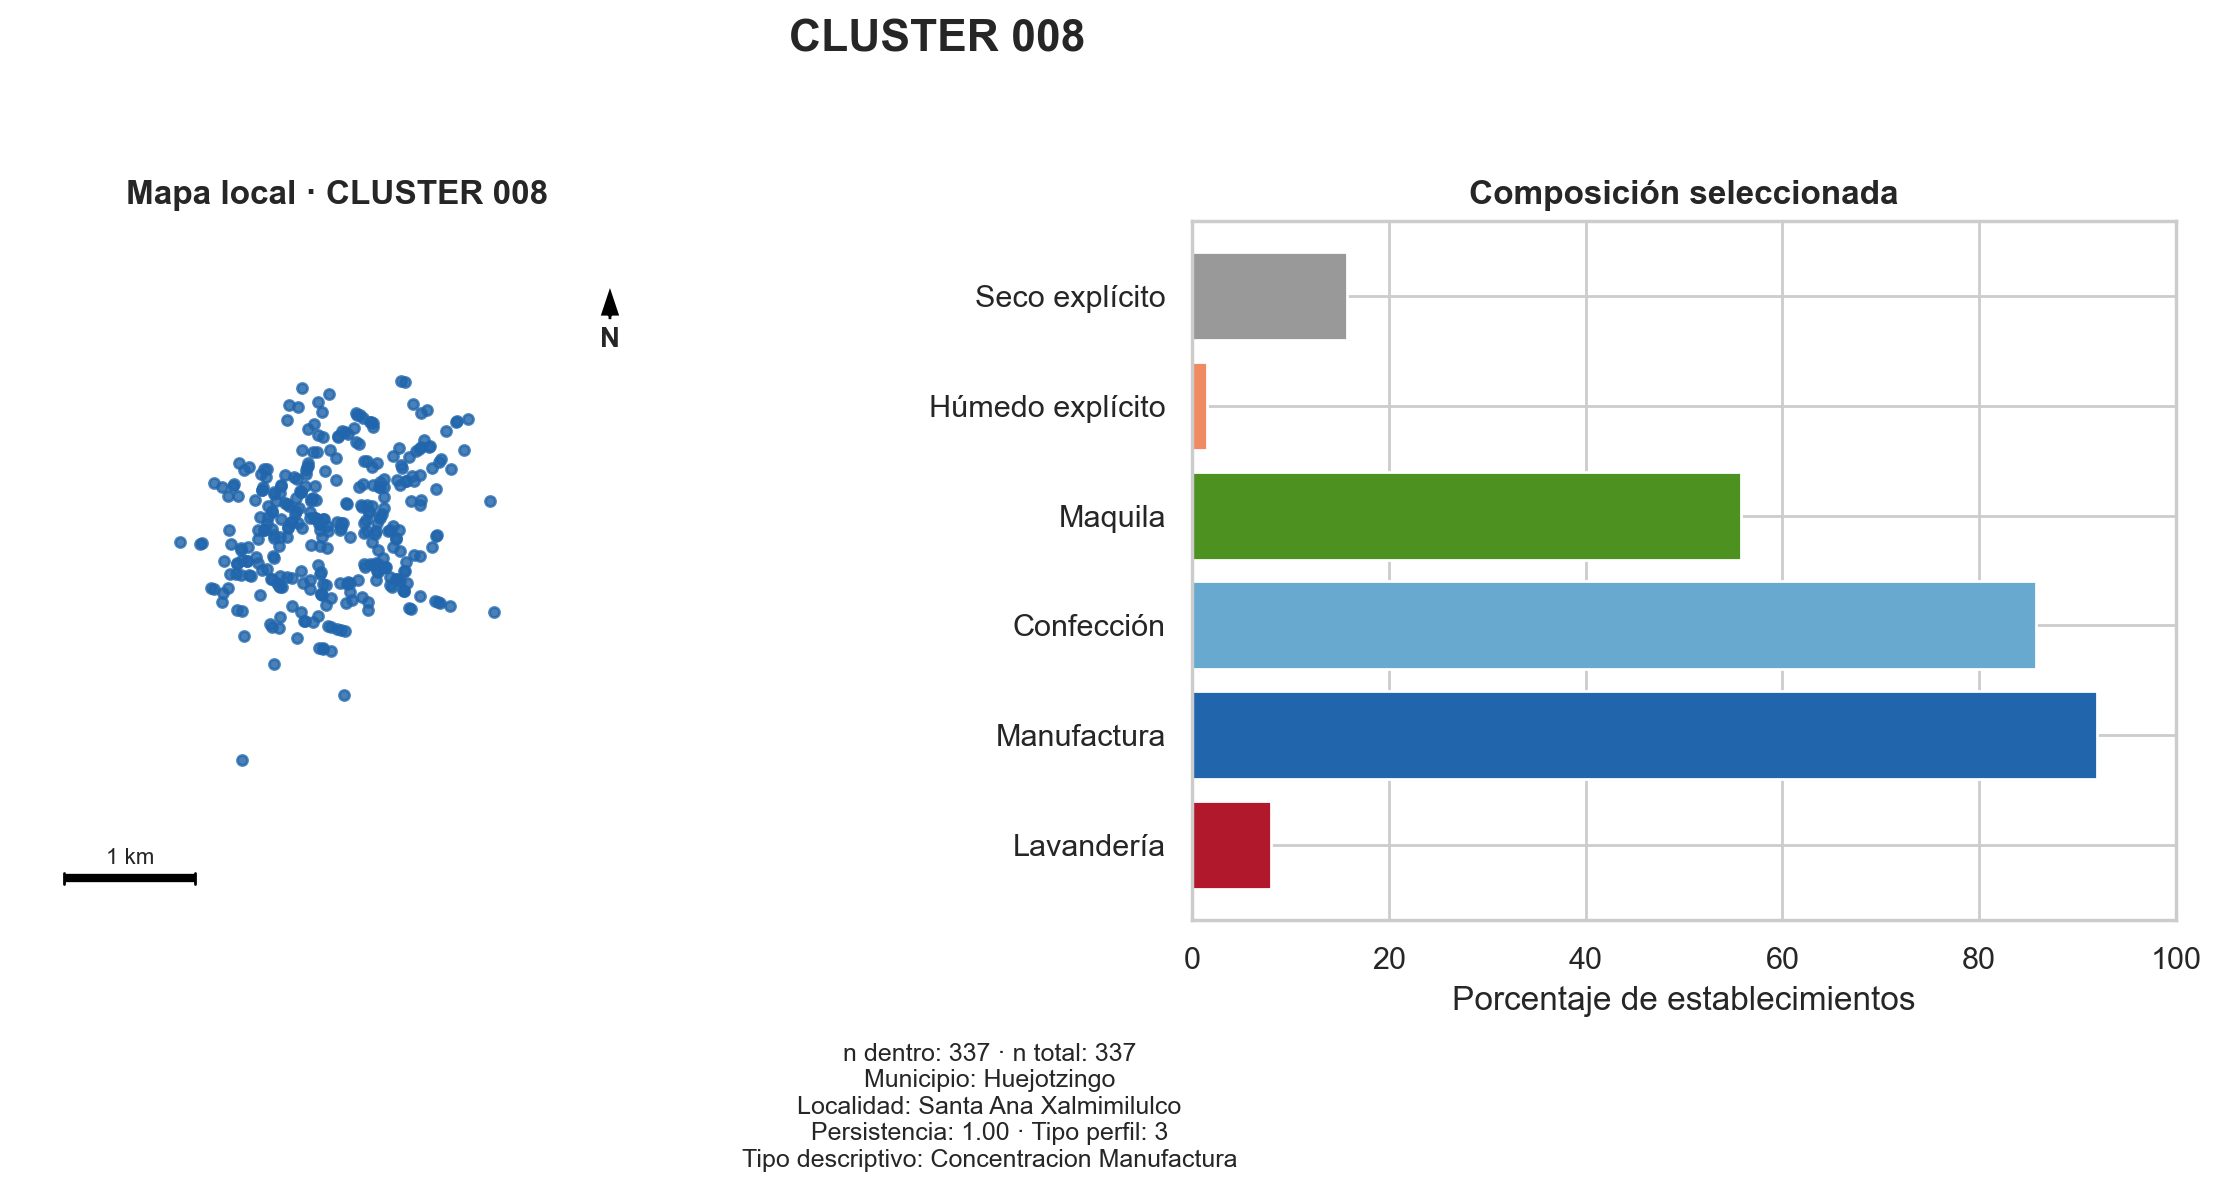
\includegraphics[width=\textwidth]{cluster_008.png}\end{center}
\begin{tabular}{p{0.31\textwidth}p{0.62\textwidth}}
\toprule
Establecimientos & 337 dentro; 0 fuera; 337 total\\
Área convexa & 4.70 km$^2$\\
Persistencia & 1.000\\
Municipio/localidad dominante & Huejotzingo / Santa Ana Xalmimilulco\\
Lavandería / manufactura & 8.0\% / 92.0\%\\
Confección / maquila & 85.8\% / 55.8\%\\
Húmedo / seco explícito & 1.5\% / 15.7\%\\
Tipología de perfil & 3.0\\
Rasgos distintivos & senal\_mezclilla\_o\_pantalon (lift 8.91) | senal\_pantalon (lift 9.79) | maquila (lift 3.80) | actividad\_confeccion (lift 2.20) | scian\_textil (lift 1.52)\\
Advertencia & Perfil descriptivo multilabel; no prueba relaciones productivas ni ambientales.\\
\bottomrule
\end{tabular}
\clearpage

\section*{Cluster 009}
\addcontentsline{toc}{section}{Cluster 009}
\begin{center}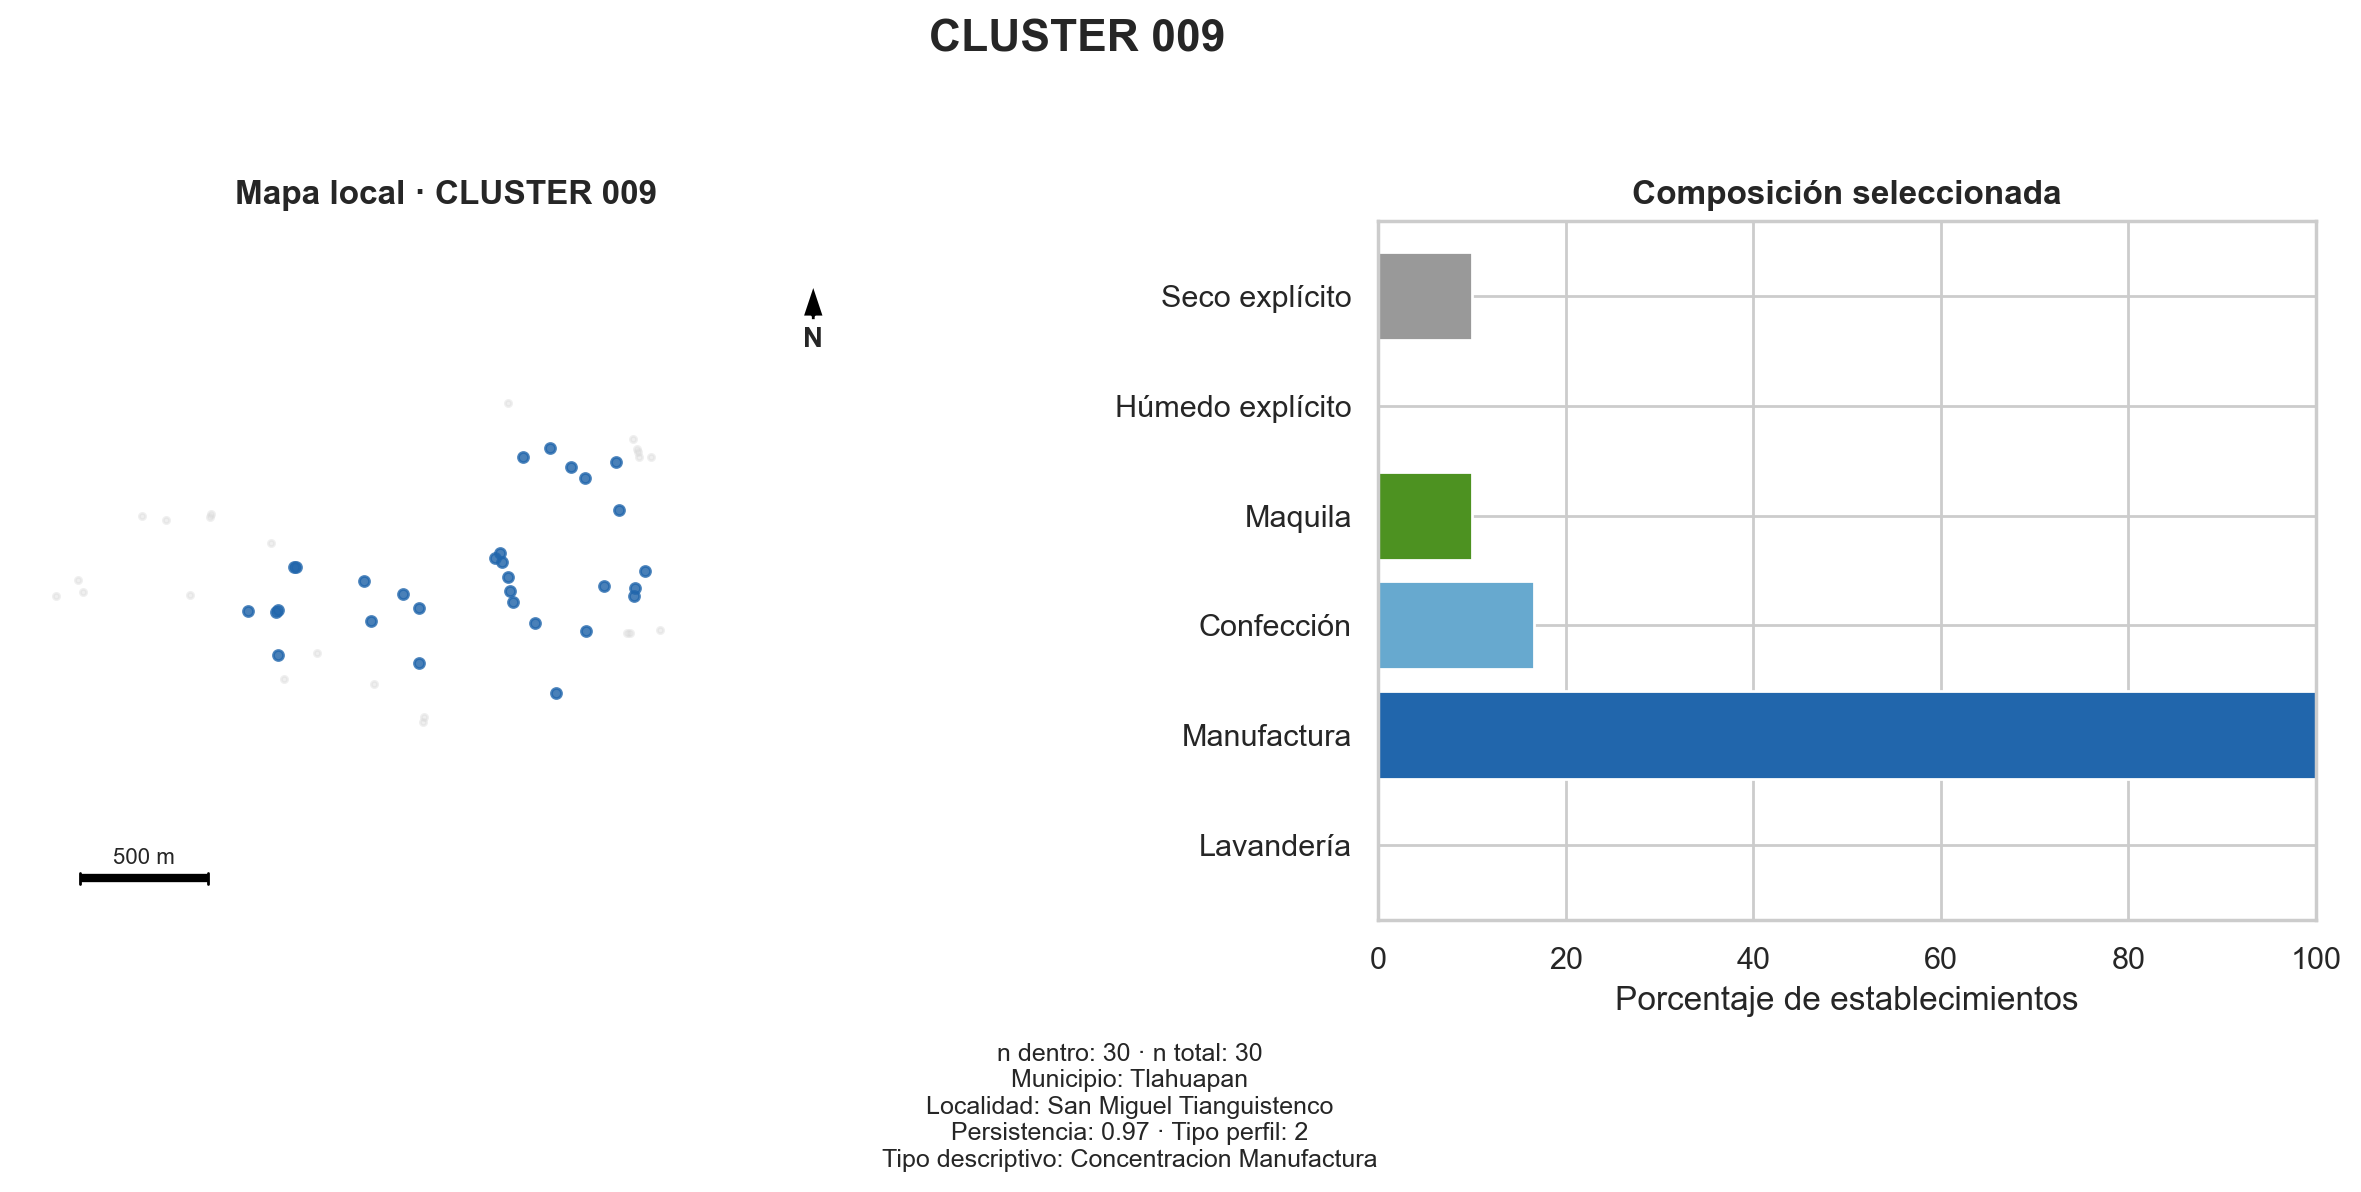
\includegraphics[width=\textwidth]{cluster_009.png}\end{center}
\begin{tabular}{p{0.31\textwidth}p{0.62\textwidth}}
\toprule
Establecimientos & 30 dentro; 0 fuera; 30 total\\
Área convexa & 0.94 km$^2$\\
Persistencia & 0.973\\
Municipio/localidad dominante & Tlahuapan / San Miguel Tianguistenco\\
Lavandería / manufactura & 0.0\% / 100.0\%\\
Confección / maquila & 16.7\% / 10.0\%\\
Húmedo / seco explícito & 0.0\% / 10.0\%\\
Tipología de perfil & 2.0\\
Rasgos distintivos & actividad\_tejido\_hilado (lift 8.94) | scian\_textil (lift 1.65)\\
Advertencia & Perfil descriptivo multilabel; no prueba relaciones productivas ni ambientales.\\
\bottomrule
\end{tabular}
\clearpage

\section*{Cluster 010}
\addcontentsline{toc}{section}{Cluster 010}
\begin{center}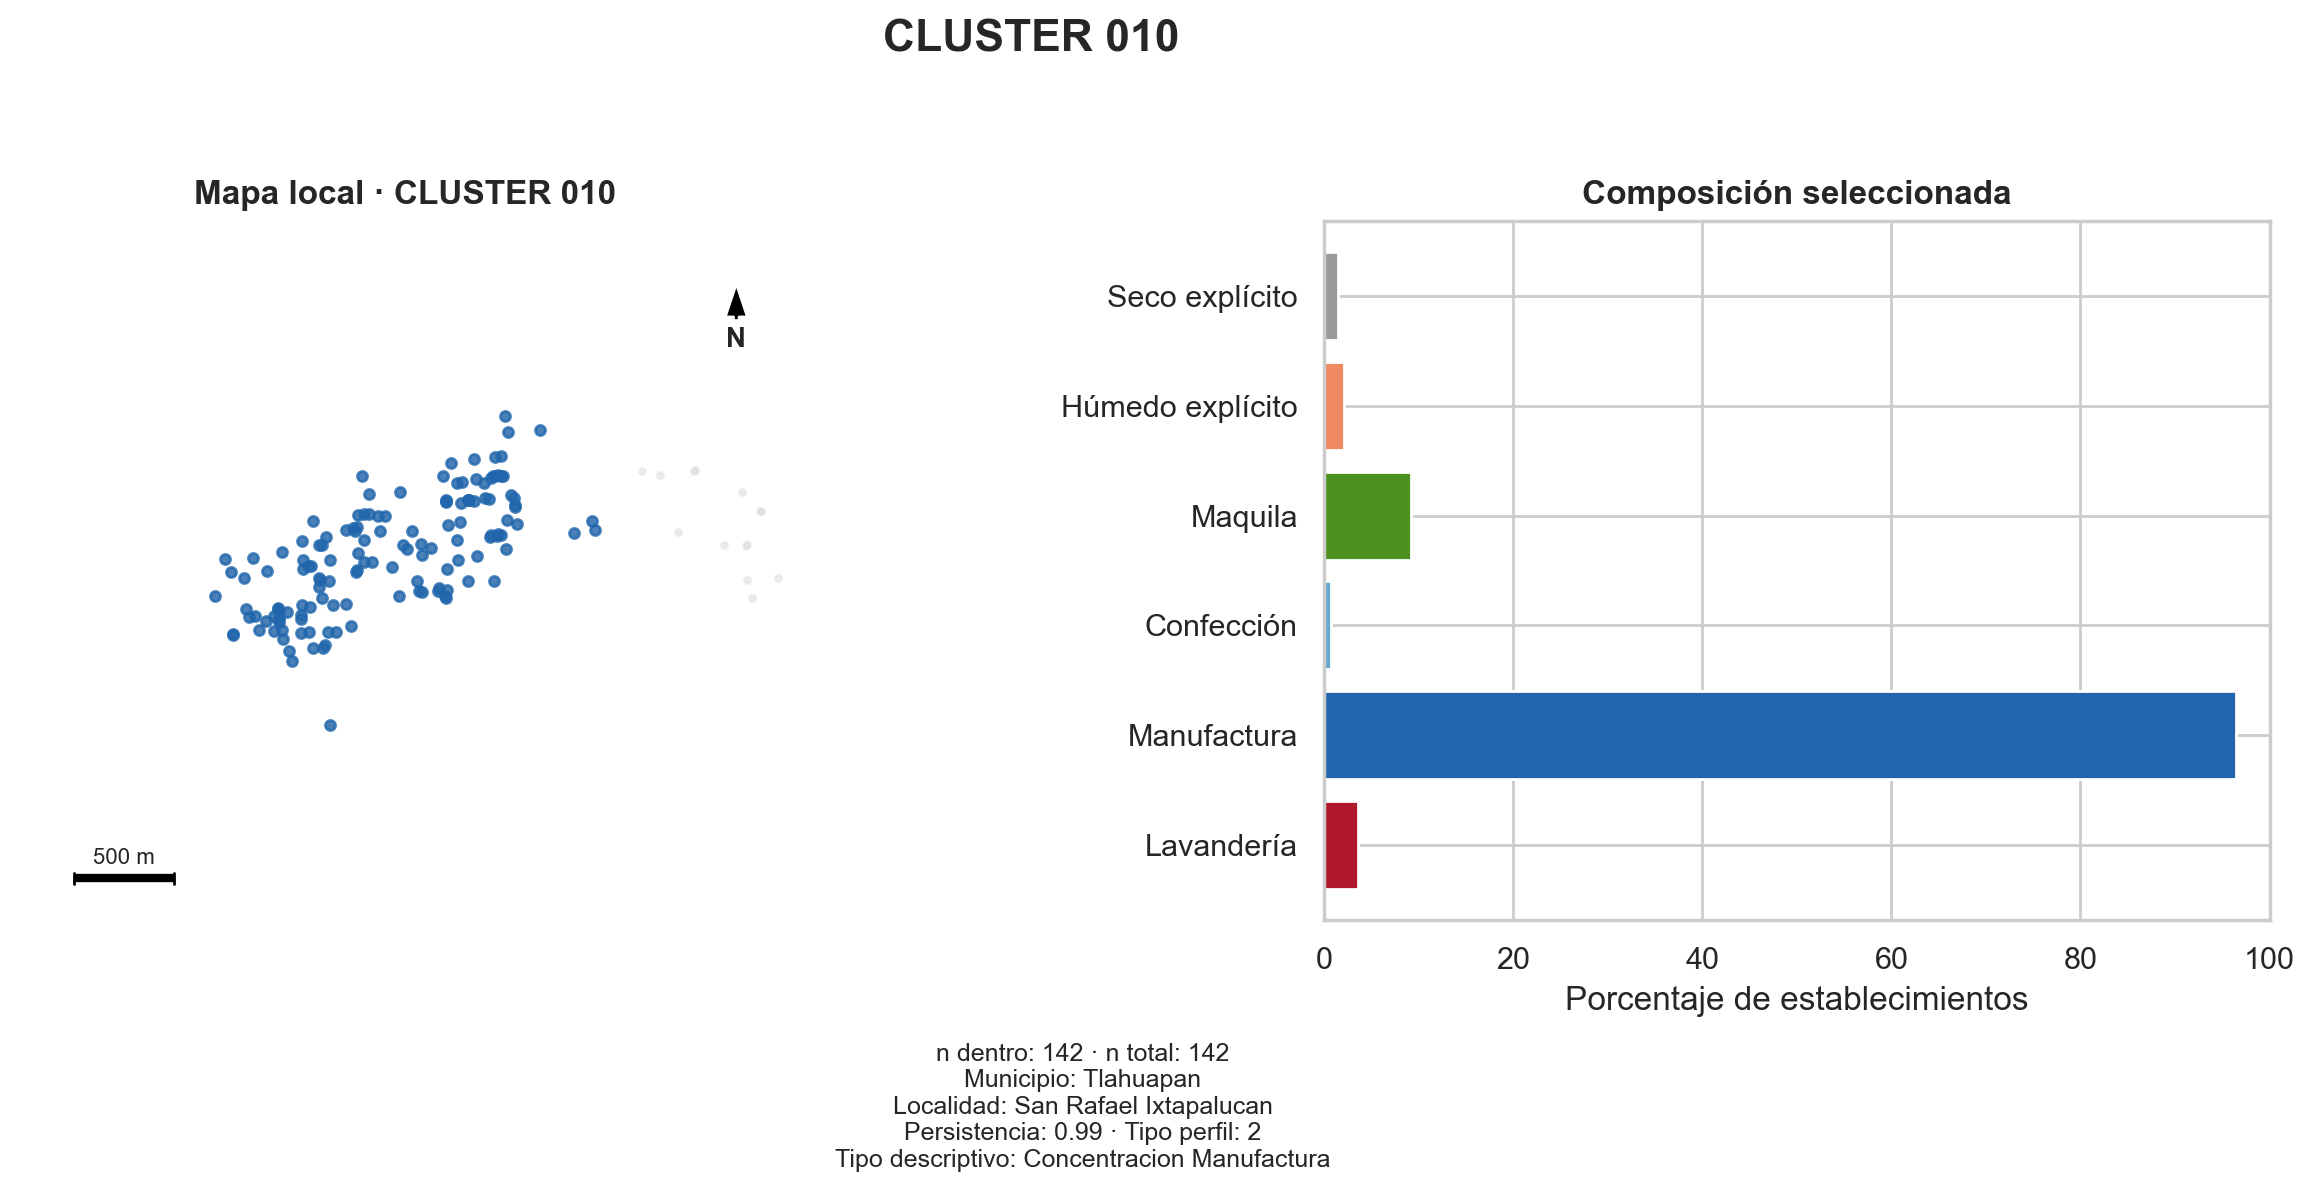
\includegraphics[width=\textwidth]{cluster_010.png}\end{center}
\begin{tabular}{p{0.31\textwidth}p{0.62\textwidth}}
\toprule
Establecimientos & 142 dentro; 0 fuera; 142 total\\
Área convexa & 1.56 km$^2$\\
Persistencia & 0.994\\
Municipio/localidad dominante & Tlahuapan / San Rafael Ixtapalucan\\
Lavandería / manufactura & 3.5\% / 96.5\%\\
Confección / maquila & 0.7\% / 9.2\%\\
Húmedo / seco explícito & 2.1\% / 1.4\%\\
Tipología de perfil & 2.0\\
Rasgos distintivos & actividad\_tejido\_hilado (lift 10.62) | scian\_textil (lift 1.60) | produccion (lift 1.73)\\
Advertencia & Perfil descriptivo multilabel; no prueba relaciones productivas ni ambientales.\\
\bottomrule
\end{tabular}
\clearpage

\section*{Cluster 011}
\addcontentsline{toc}{section}{Cluster 011}
\begin{center}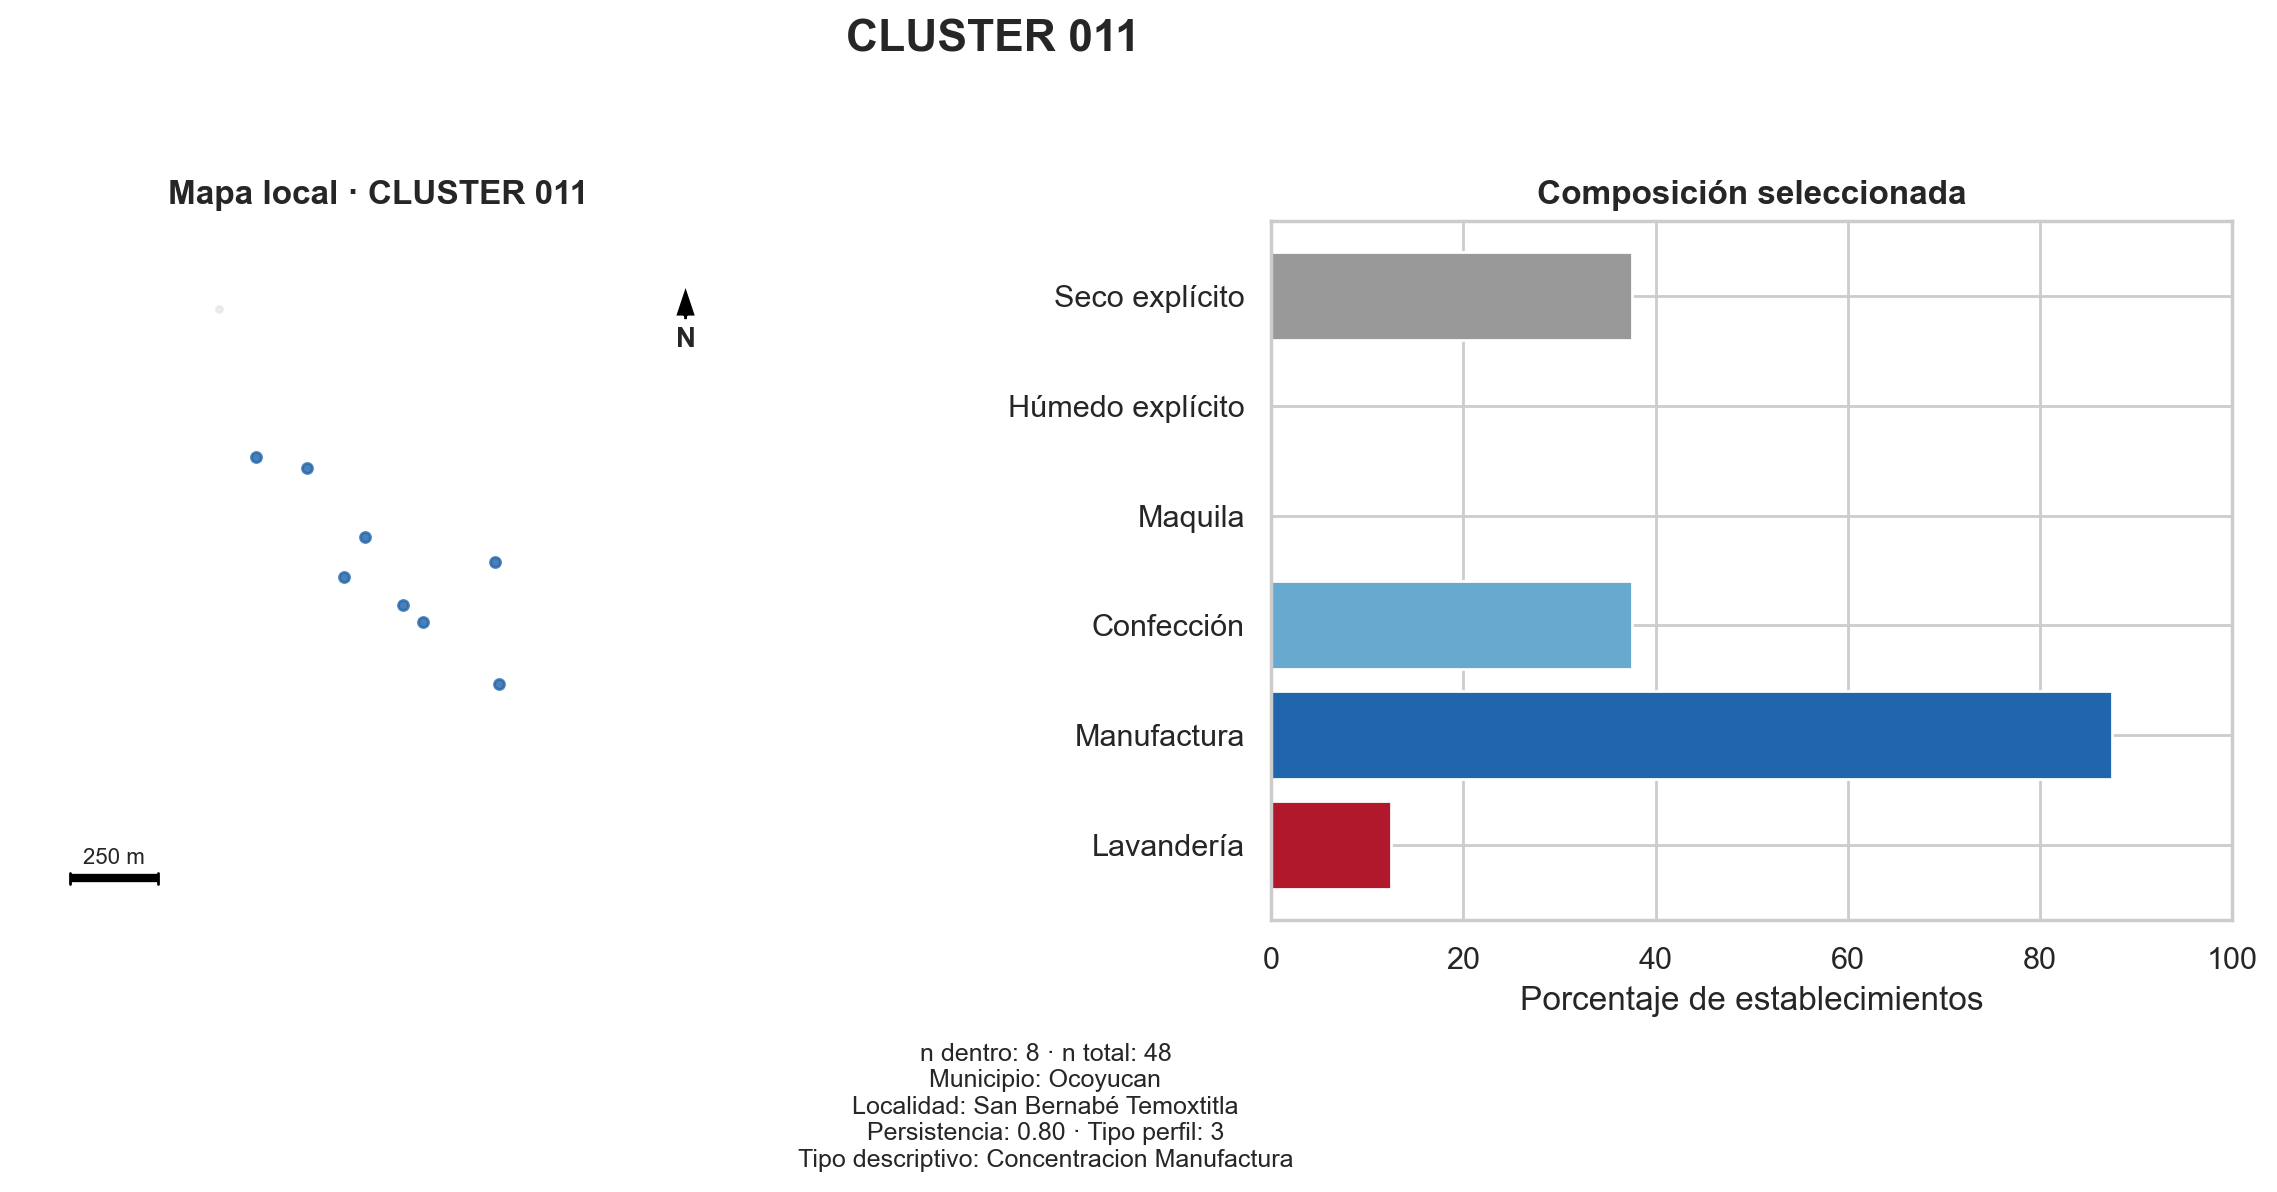
\includegraphics[width=\textwidth]{cluster_011.png}\end{center}
\begin{tabular}{p{0.31\textwidth}p{0.62\textwidth}}
\toprule
Establecimientos & 8 dentro; 40 fuera; 48 total\\
Área convexa & 2.92 km$^2$\\
Persistencia & 0.800\\
Municipio/localidad dominante & Ocoyucan / San Bernabé Temoxtitla\\
Lavandería / manufactura & 12.5\% / 87.5\%\\
Confección / maquila & 37.5\% / 0.0\%\\
Húmedo / seco explícito & 0.0\% / 37.5\%\\
Tipología de perfil & 3.0\\
Rasgos distintivos & Sin rasgos que cumplan todos los umbrales conservadores\\
Advertencia & Perfil descriptivo multilabel; no prueba relaciones productivas ni ambientales.\\
\bottomrule
\end{tabular}
\clearpage

\section*{Cluster 012}
\addcontentsline{toc}{section}{Cluster 012}
\begin{center}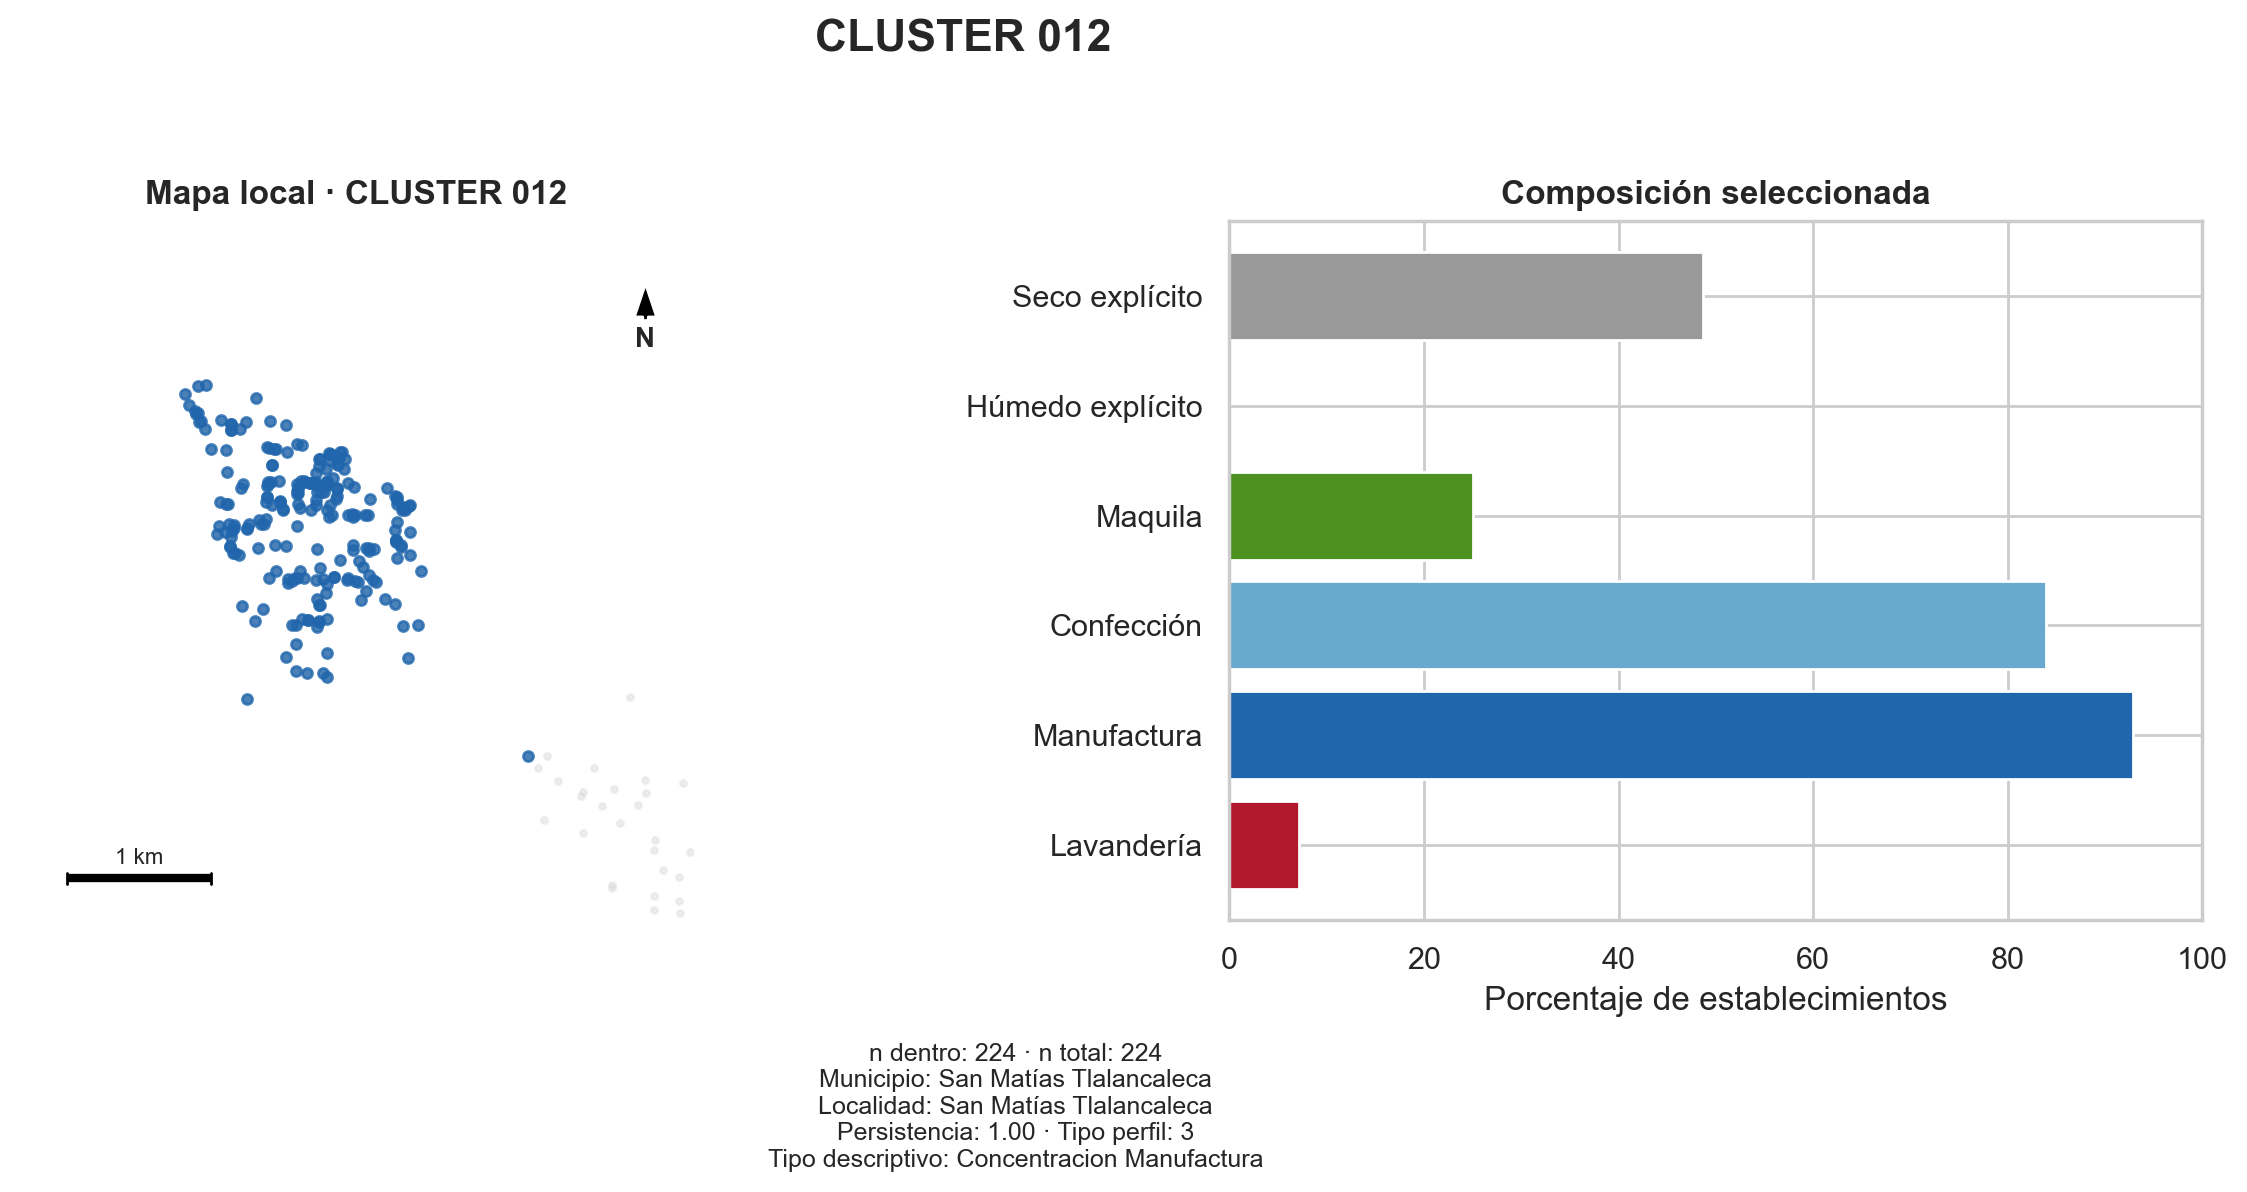
\includegraphics[width=\textwidth]{cluster_012.png}\end{center}
\begin{tabular}{p{0.31\textwidth}p{0.62\textwidth}}
\toprule
Establecimientos & 224 dentro; 0 fuera; 224 total\\
Área convexa & 3.25 km$^2$\\
Persistencia & 0.998\\
Municipio/localidad dominante & San Matías Tlalancaleca / San Matías Tlalancaleca\\
Lavandería / manufactura & 7.1\% / 92.9\%\\
Confección / maquila & 83.9\% / 25.0\%\\
Húmedo / seco explícito & 0.0\% / 48.7\%\\
Tipología de perfil & 3.0\\
Rasgos distintivos & textil (lift 2.64) | actividad\_confeccion (lift 2.15) | proceso\_seco\_explicito (lift 3.03) | scian\_textil (lift 1.54) | senal\_mezclilla\_o\_pantalon (lift 3.03)\\
Advertencia & Perfil descriptivo multilabel; no prueba relaciones productivas ni ambientales.\\
\bottomrule
\end{tabular}
\clearpage

\section*{Cluster 013}
\addcontentsline{toc}{section}{Cluster 013}
\begin{center}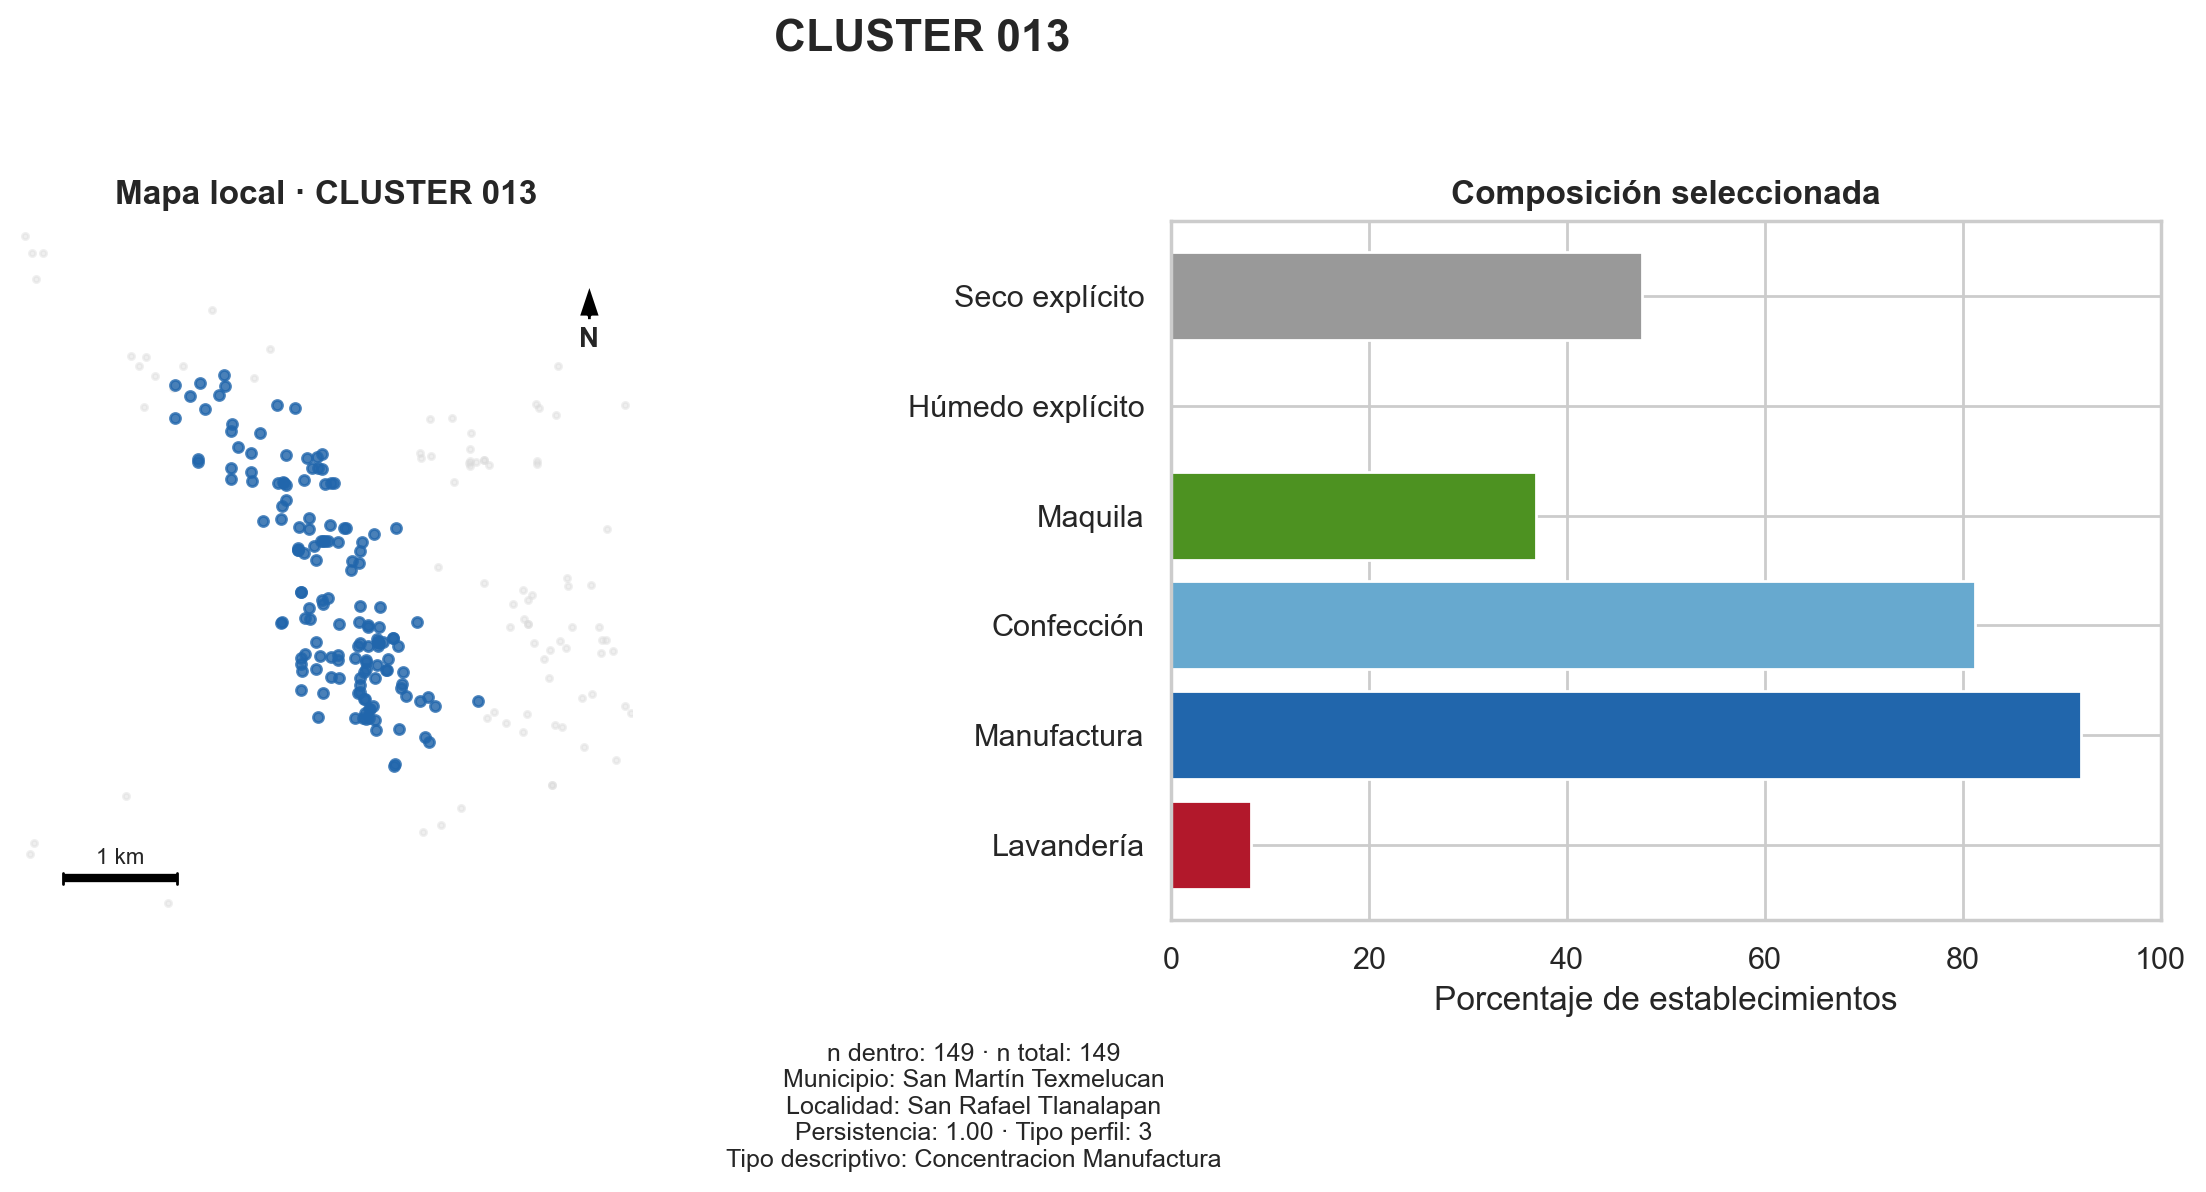
\includegraphics[width=\textwidth]{cluster_013.png}\end{center}
\begin{tabular}{p{0.31\textwidth}p{0.62\textwidth}}
\toprule
Establecimientos & 149 dentro; 0 fuera; 149 total\\
Área convexa & 4.25 km$^2$\\
Persistencia & 0.997\\
Municipio/localidad dominante & San Martín Texmelucan / San Rafael Tlanalapan\\
Lavandería / manufactura & 8.1\% / 91.9\%\\
Confección / maquila & 81.2\% / 36.9\%\\
Húmedo / seco explícito & 0.0\% / 47.7\%\\
Tipología de perfil & 3.0\\
Rasgos distintivos & actividad\_confeccion (lift 2.08) | proceso\_seco\_explicito (lift 2.97) | textil (lift 2.13) | scian\_textil (lift 1.52) | maquila (lift 2.51)\\
Advertencia & Perfil descriptivo multilabel; no prueba relaciones productivas ni ambientales.\\
\bottomrule
\end{tabular}
\clearpage

\section*{Cluster 014}
\addcontentsline{toc}{section}{Cluster 014}
\begin{center}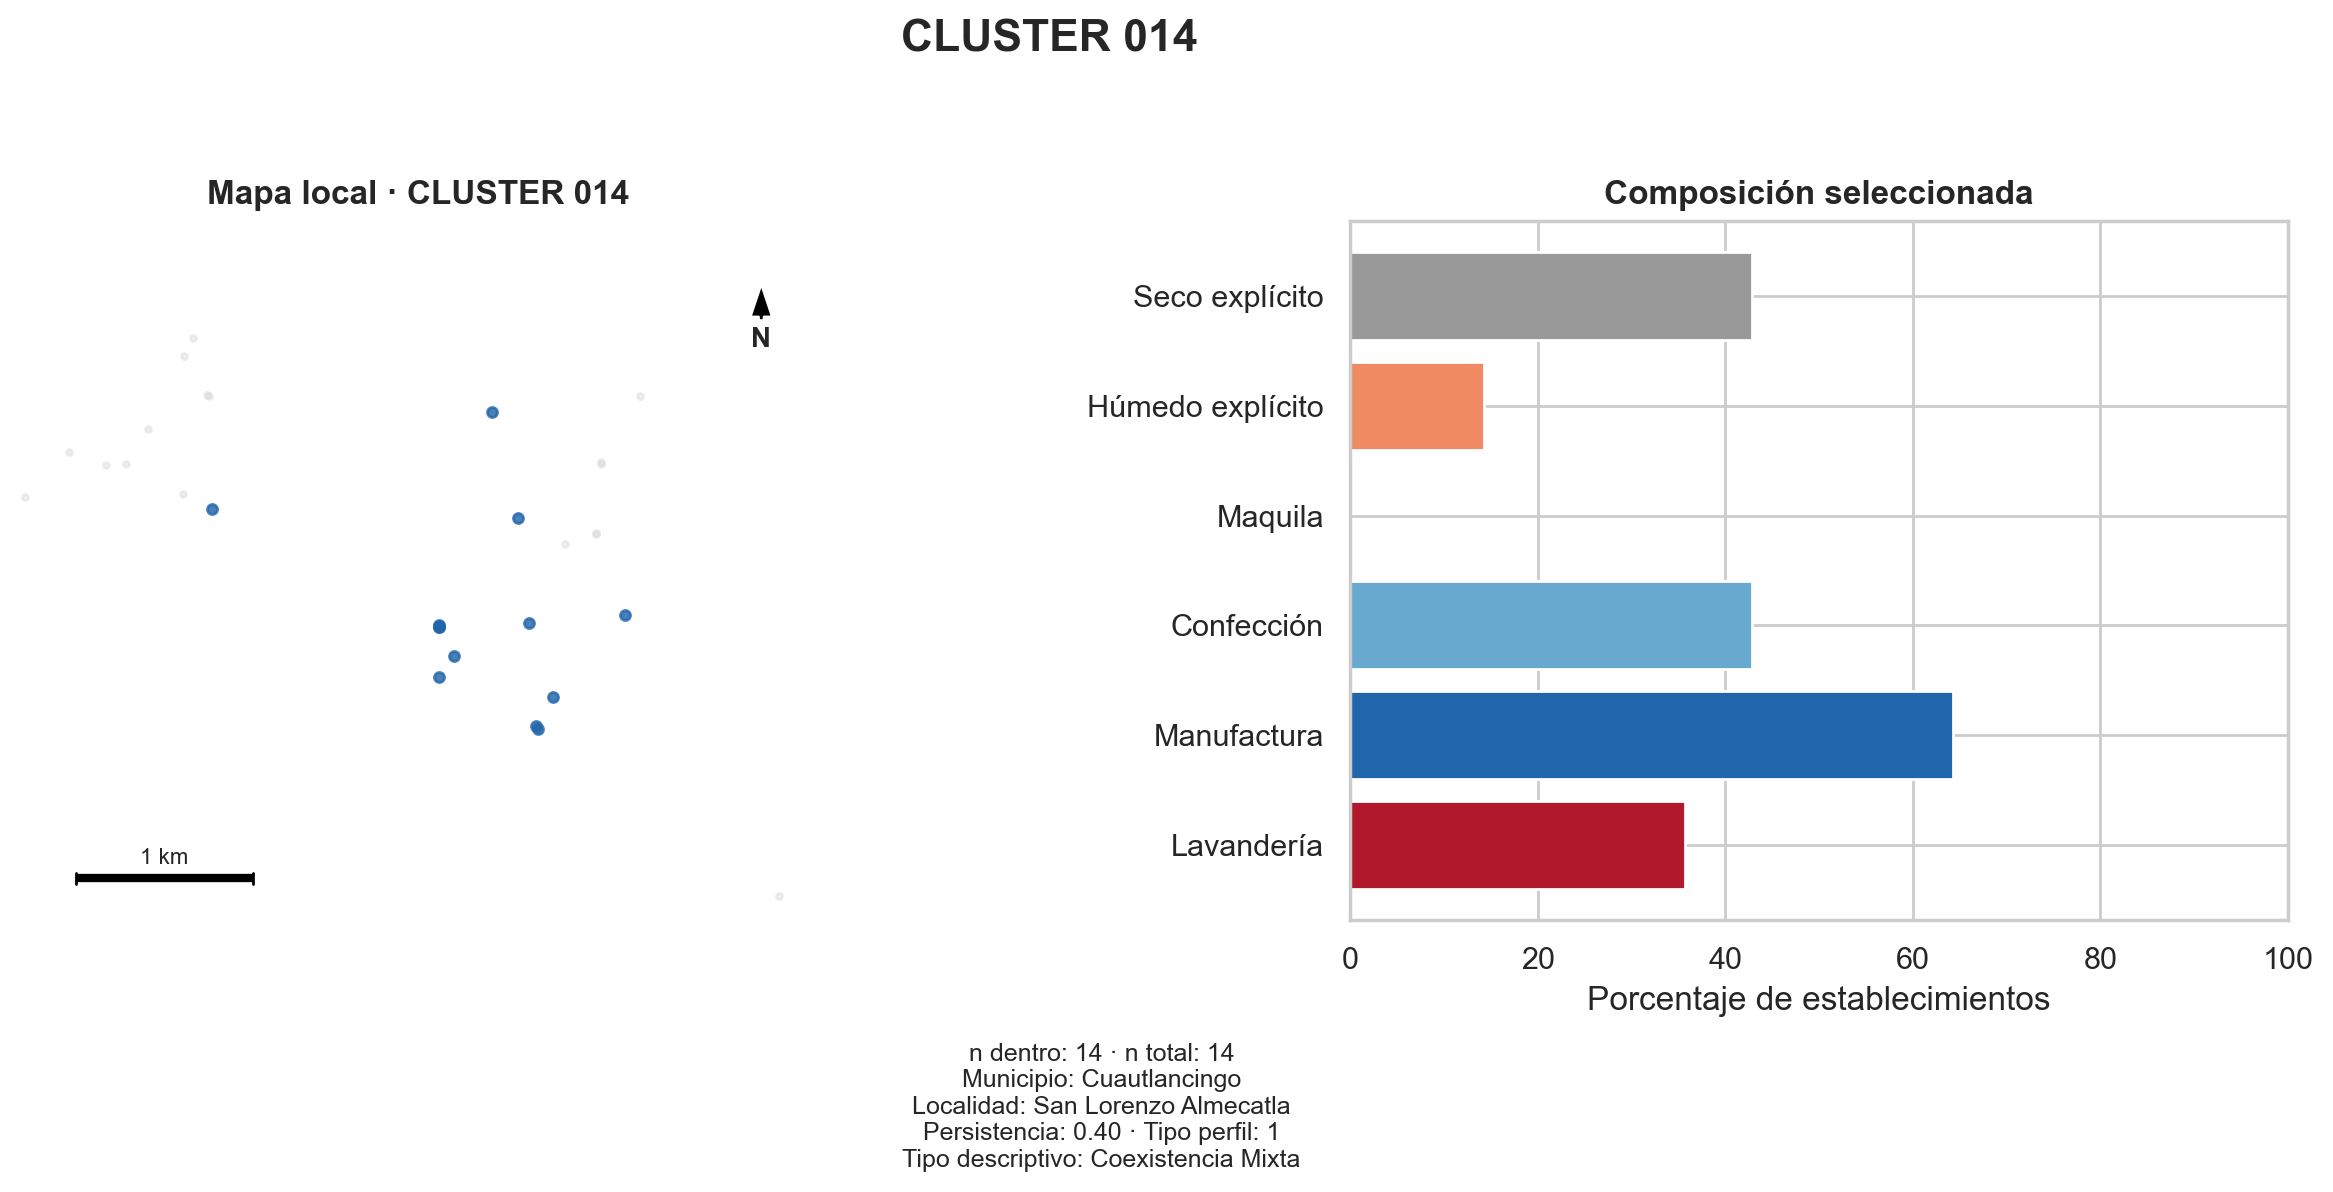
\includegraphics[width=\textwidth]{cluster_014.png}\end{center}
\begin{tabular}{p{0.31\textwidth}p{0.62\textwidth}}
\toprule
Establecimientos & 14 dentro; 0 fuera; 14 total\\
Área convexa & 2.09 km$^2$\\
Persistencia & 0.400\\
Municipio/localidad dominante & Cuautlancingo / San Lorenzo Almecatla\\
Lavandería / manufactura & 35.7\% / 64.3\%\\
Confección / maquila & 42.9\% / 0.0\%\\
Húmedo / seco explícito & 14.3\% / 42.9\%\\
Tipología de perfil & 1.0\\
Rasgos distintivos & proceso\_seco\_explicito (lift 2.67)\\
Advertencia & Perfil descriptivo multilabel; no prueba relaciones productivas ni ambientales.\\
\bottomrule
\end{tabular}
\clearpage

\section*{Cluster 015}
\addcontentsline{toc}{section}{Cluster 015}
\begin{center}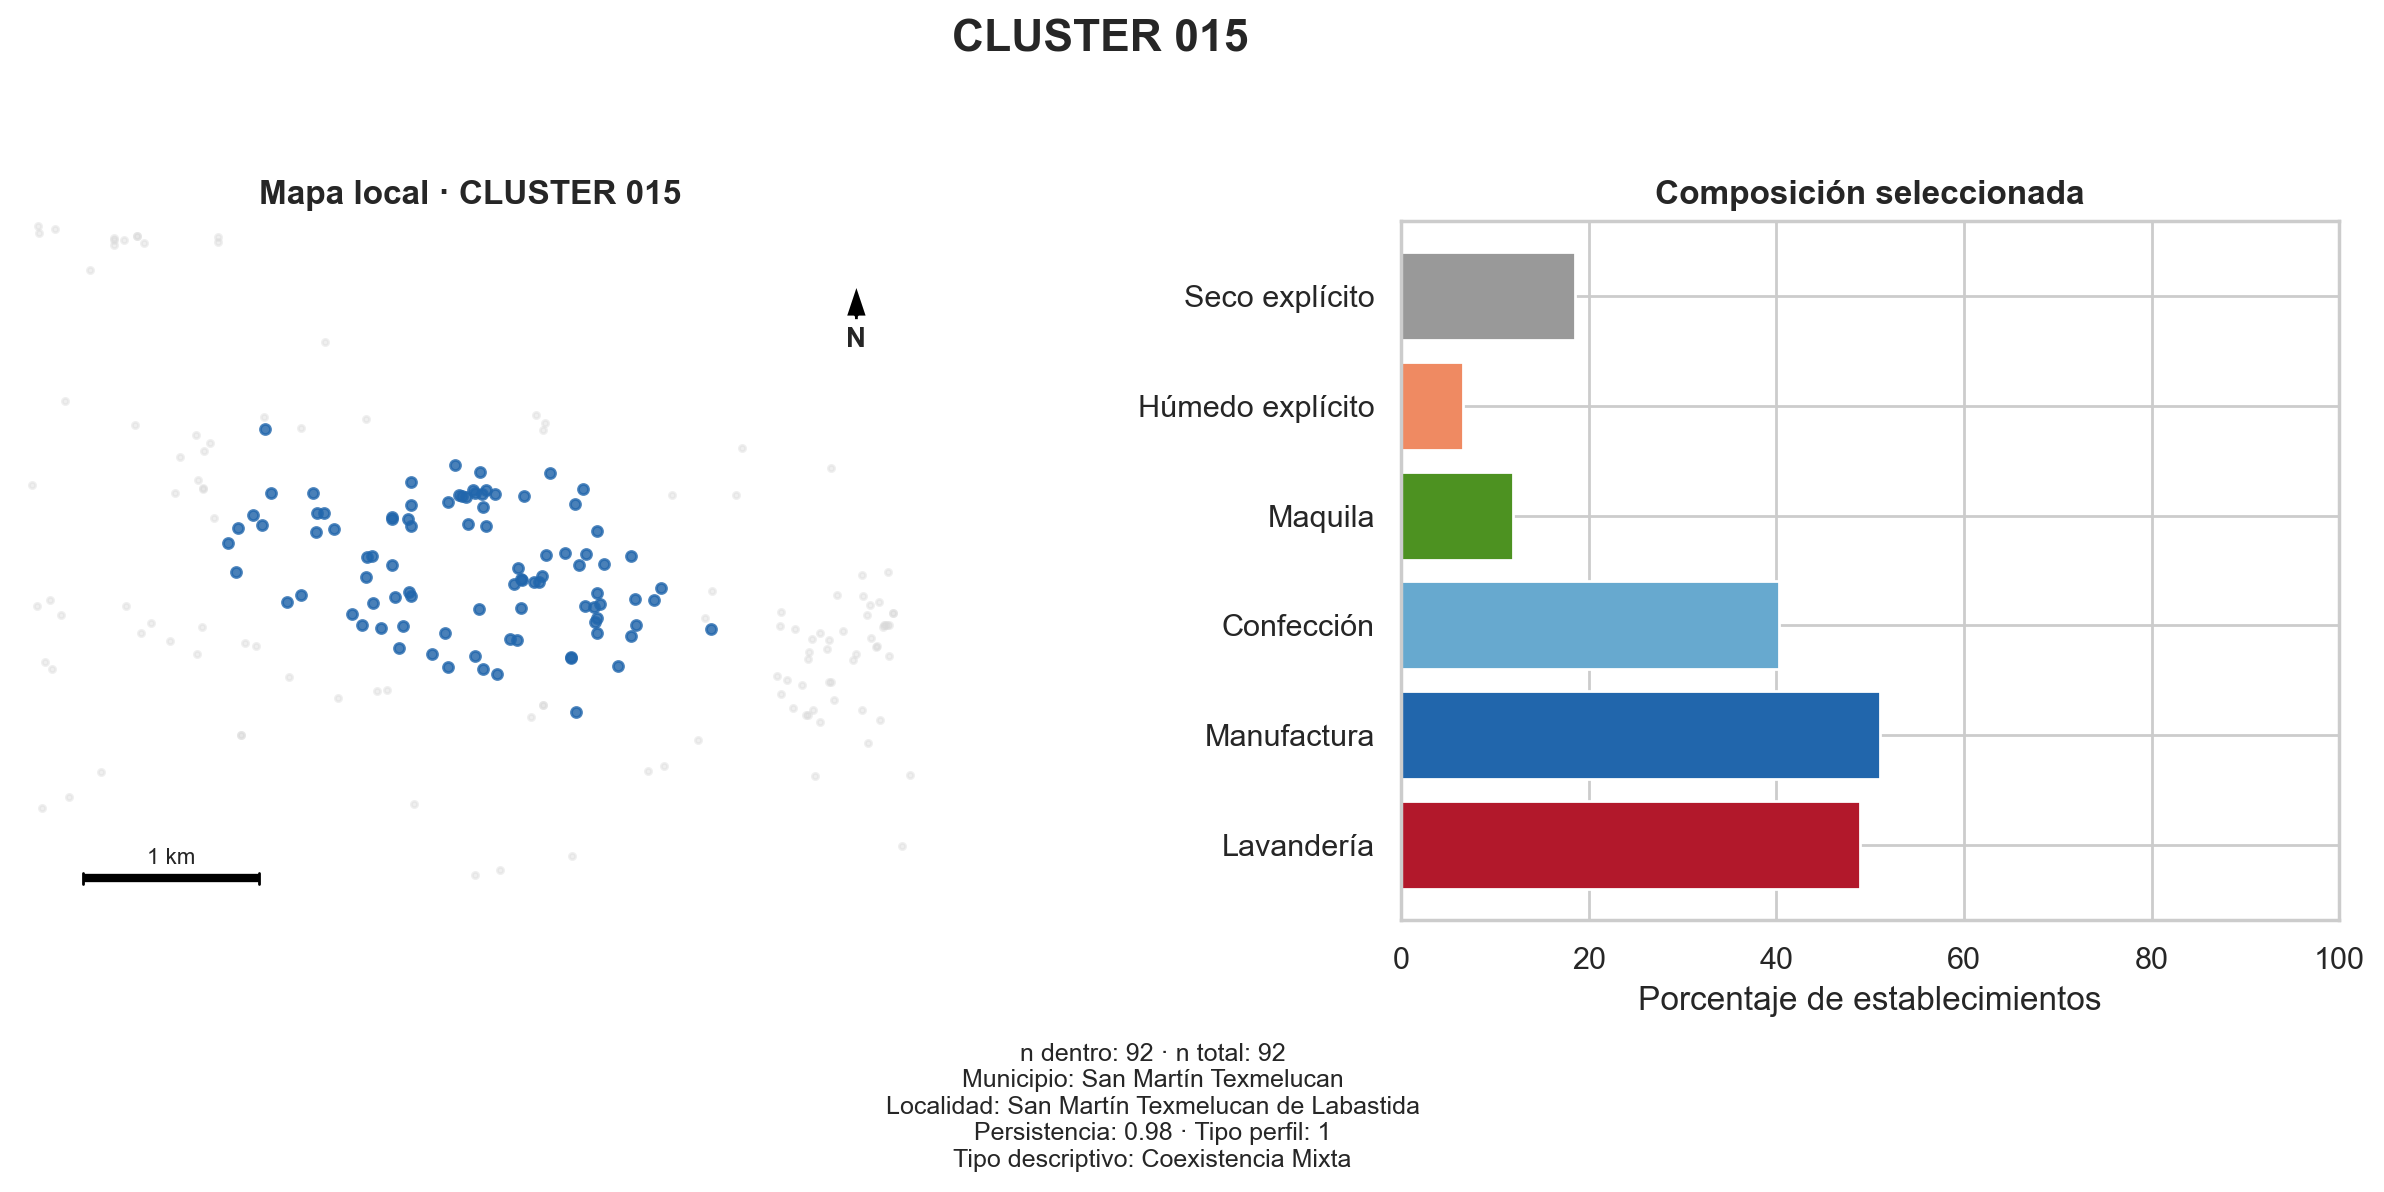
\includegraphics[width=\textwidth]{cluster_015.png}\end{center}
\begin{tabular}{p{0.31\textwidth}p{0.62\textwidth}}
\toprule
Establecimientos & 92 dentro; 0 fuera; 92 total\\
Área convexa & 2.63 km$^2$\\
Persistencia & 0.978\\
Municipio/localidad dominante & San Martín Texmelucan / San Martín Texmelucan de Labastida\\
Lavandería / manufactura & 48.9\% / 51.1\%\\
Confección / maquila & 40.2\% / 12.0\%\\
Húmedo / seco explícito & 6.5\% / 18.5\%\\
Tipología de perfil & 1.0\\
Rasgos distintivos & Sin rasgos que cumplan todos los umbrales conservadores\\
Advertencia & Perfil descriptivo multilabel; no prueba relaciones productivas ni ambientales.\\
\bottomrule
\end{tabular}
\clearpage

\section*{Cluster 016}
\addcontentsline{toc}{section}{Cluster 016}
\begin{center}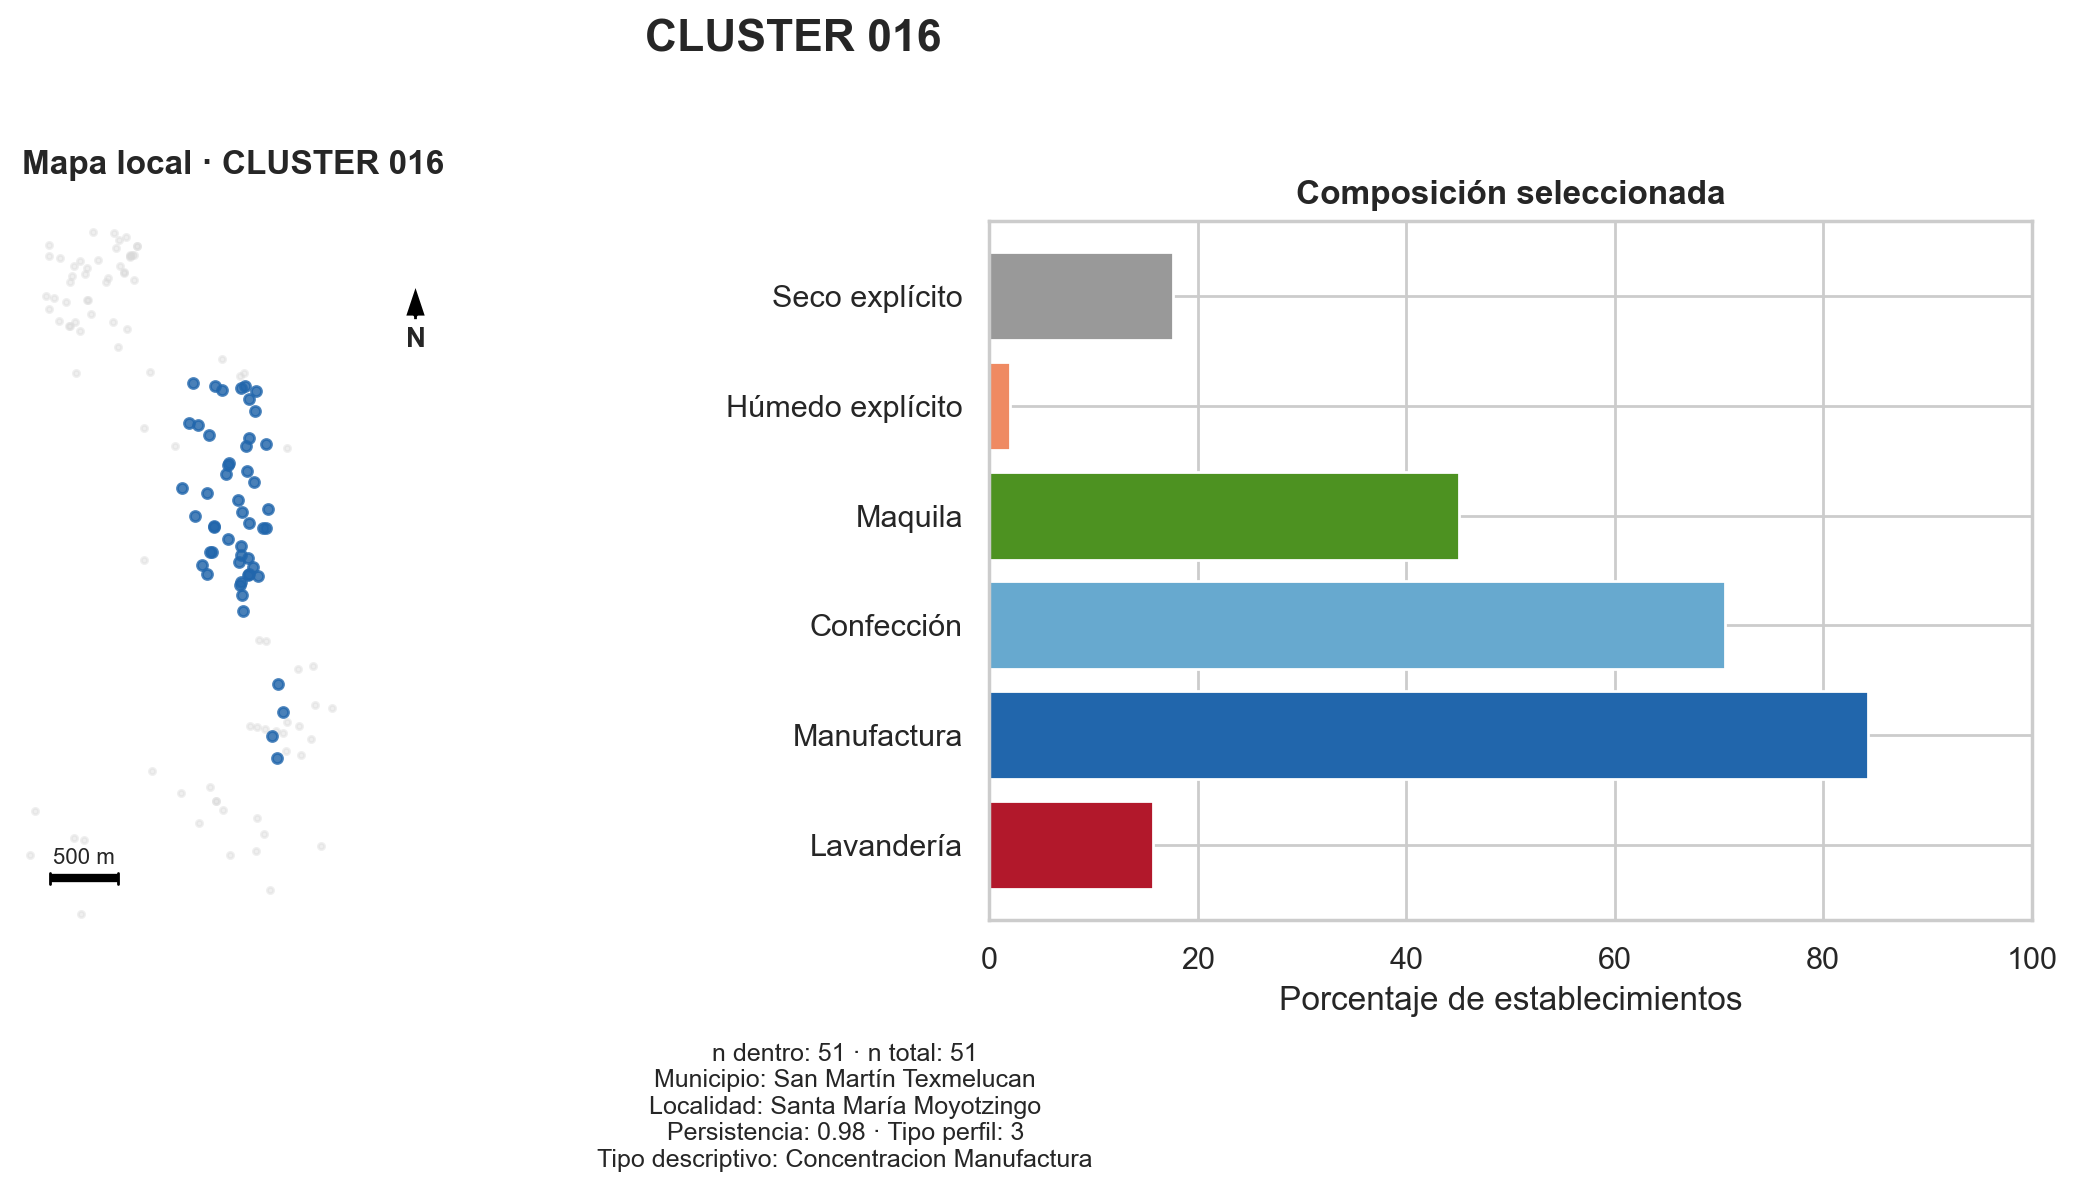
\includegraphics[width=\textwidth]{cluster_016.png}\end{center}
\begin{tabular}{p{0.31\textwidth}p{0.62\textwidth}}
\toprule
Establecimientos & 51 dentro; 0 fuera; 51 total\\
Área convexa & 1.13 km$^2$\\
Persistencia & 0.984\\
Municipio/localidad dominante & San Martín Texmelucan / Santa María Moyotzingo\\
Lavandería / manufactura & 15.7\% / 84.3\%\\
Confección / maquila & 70.6\% / 45.1\%\\
Húmedo / seco explícito & 2.0\% / 17.6\%\\
Tipología de perfil & 3.0\\
Rasgos distintivos & maquila (lift 3.07) | actividad\_confeccion (lift 1.81) | scian\_textil (lift 1.39)\\
Advertencia & Perfil descriptivo multilabel; no prueba relaciones productivas ni ambientales.\\
\bottomrule
\end{tabular}
\clearpage

\section*{Cluster 017}
\addcontentsline{toc}{section}{Cluster 017}
\begin{center}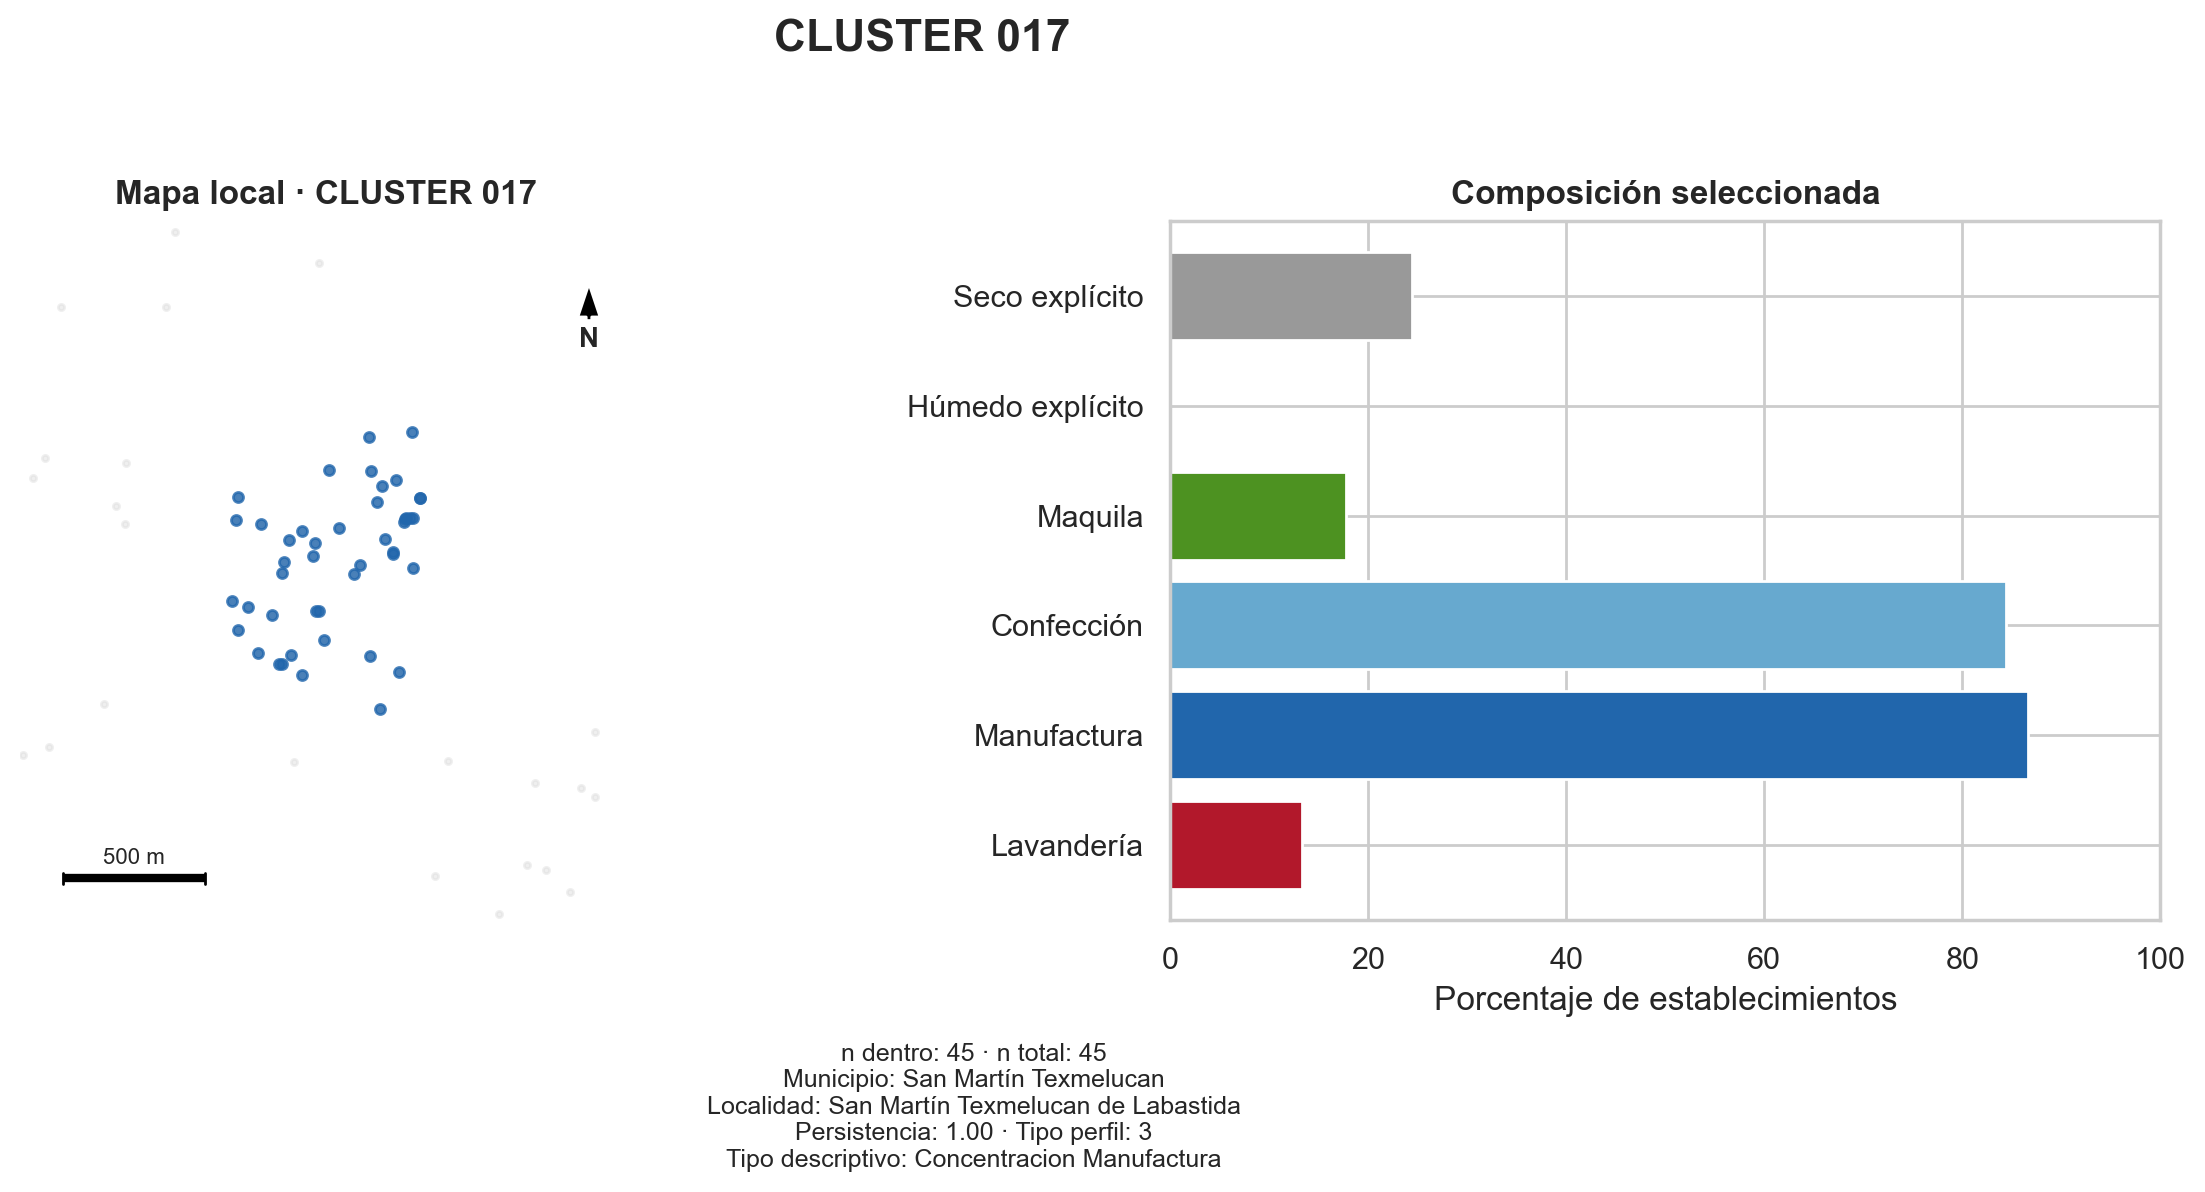
\includegraphics[width=\textwidth]{cluster_017.png}\end{center}
\begin{tabular}{p{0.31\textwidth}p{0.62\textwidth}}
\toprule
Establecimientos & 45 dentro; 0 fuera; 45 total\\
Área convexa & 0.47 km$^2$\\
Persistencia & 1.000\\
Municipio/localidad dominante & San Martín Texmelucan / San Martín Texmelucan de Labastida\\
Lavandería / manufactura & 13.3\% / 86.7\%\\
Confección / maquila & 84.4\% / 17.8\%\\
Húmedo / seco explícito & 0.0\% / 24.4\%\\
Tipología de perfil & 3.0\\
Rasgos distintivos & actividad\_confeccion (lift 2.17) | scian\_textil (lift 1.43)\\
Advertencia & Perfil descriptivo multilabel; no prueba relaciones productivas ni ambientales.\\
\bottomrule
\end{tabular}
\clearpage

\section*{Cluster 018}
\addcontentsline{toc}{section}{Cluster 018}
\begin{center}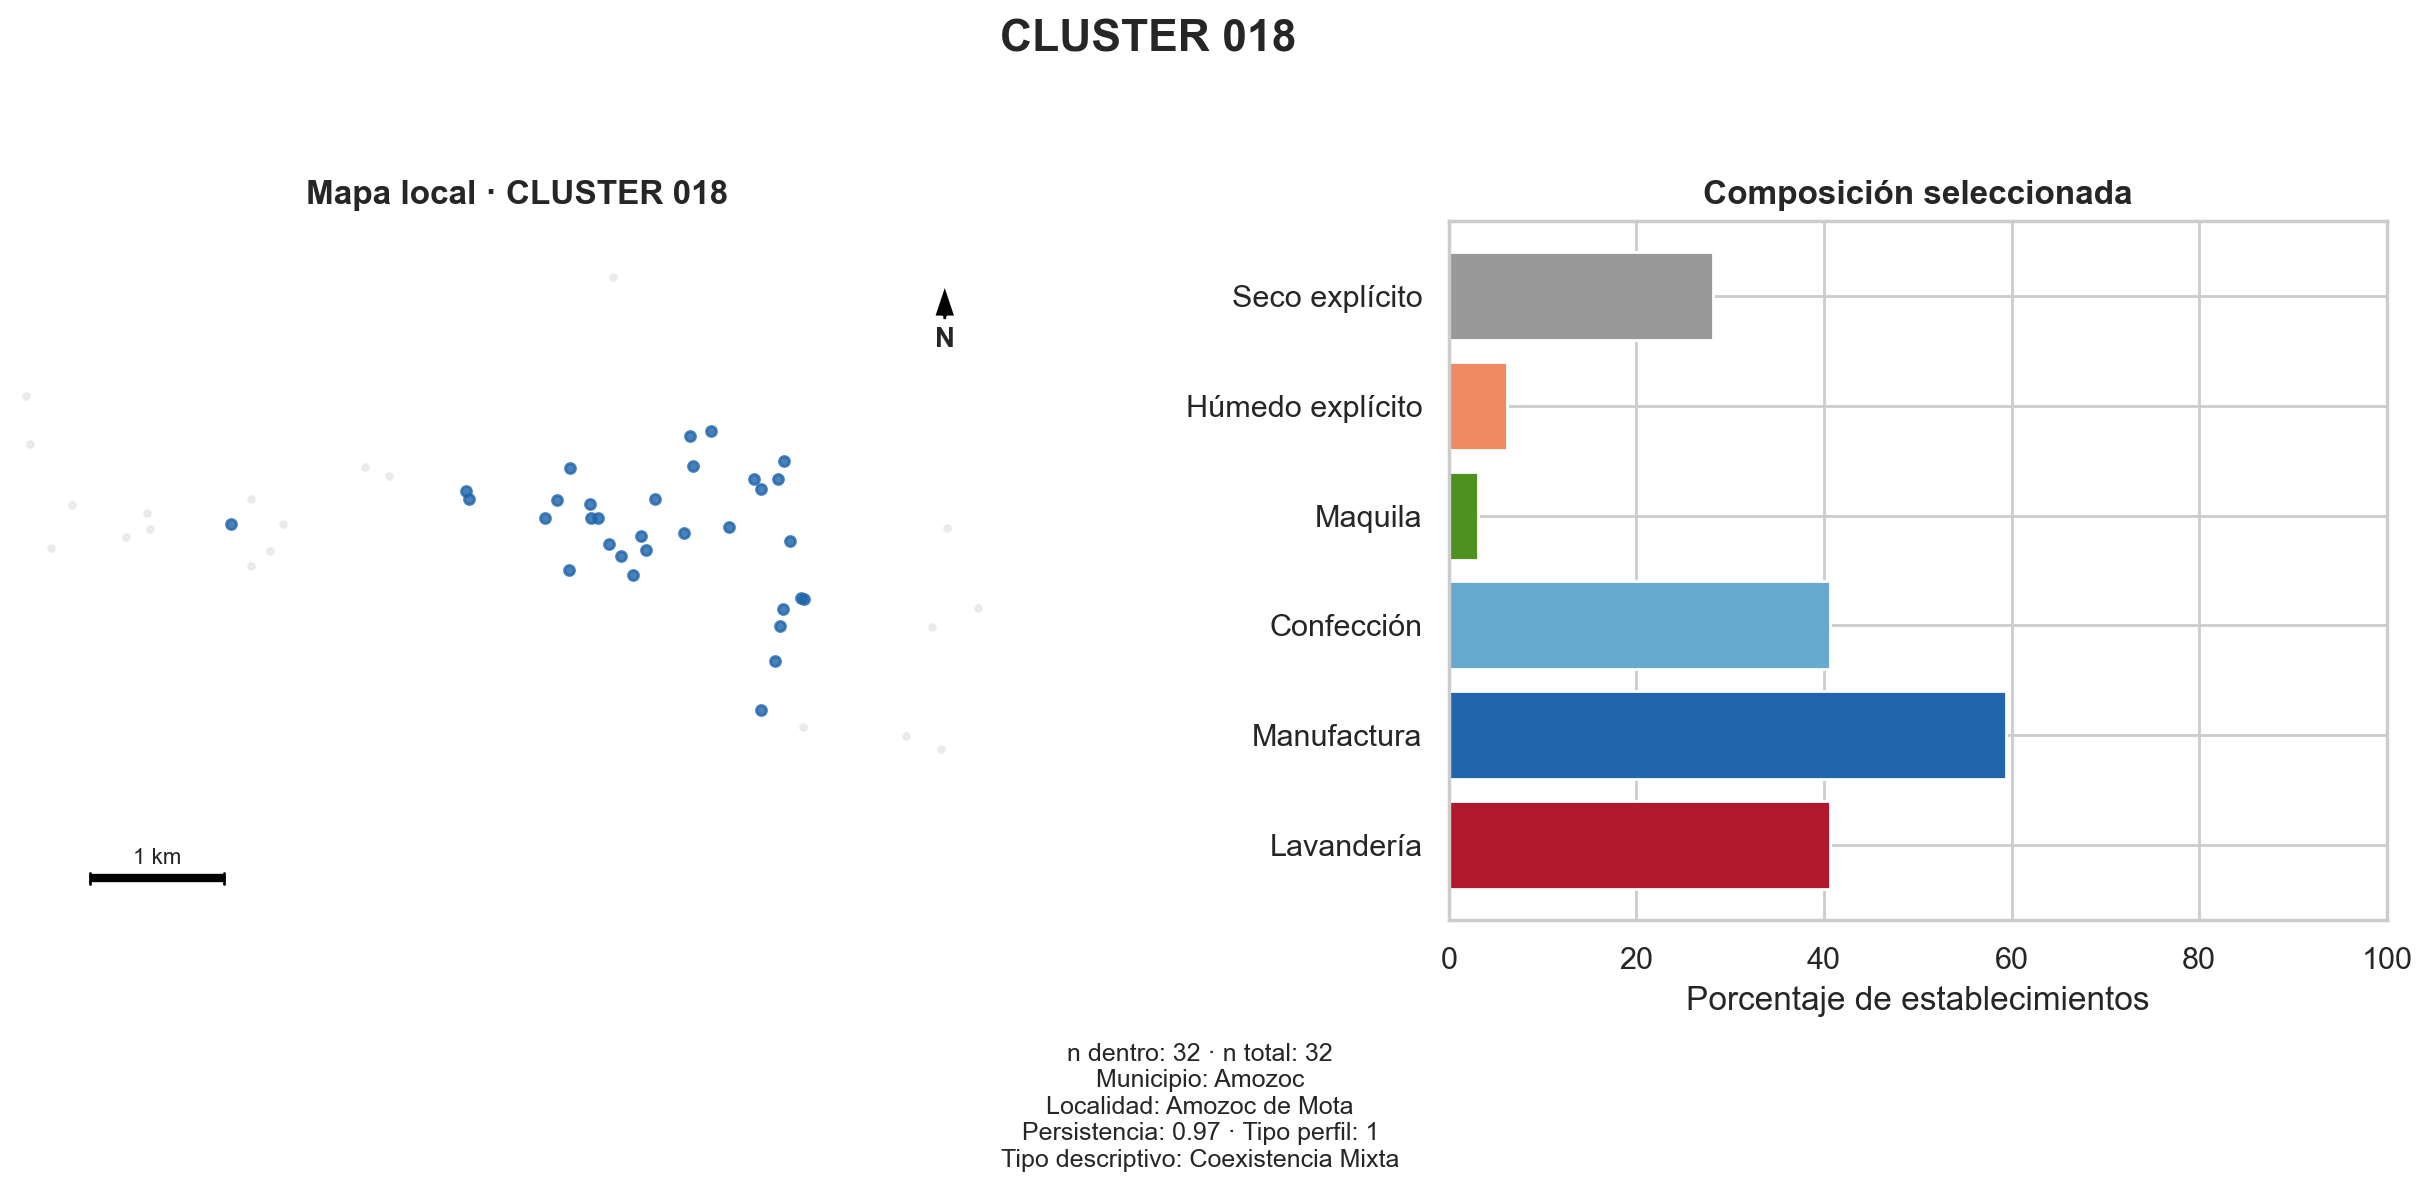
\includegraphics[width=\textwidth]{cluster_018.png}\end{center}
\begin{tabular}{p{0.31\textwidth}p{0.62\textwidth}}
\toprule
Establecimientos & 32 dentro; 0 fuera; 32 total\\
Área convexa & 4.55 km$^2$\\
Persistencia & 0.969\\
Municipio/localidad dominante & Amozoc / Amozoc de Mota\\
Lavandería / manufactura & 40.6\% / 59.4\%\\
Confección / maquila & 40.6\% / 3.1\%\\
Húmedo / seco explícito & 6.2\% / 28.1\%\\
Tipología de perfil & 1.0\\
Rasgos distintivos & textil (lift 1.89)\\
Advertencia & Perfil descriptivo multilabel; no prueba relaciones productivas ni ambientales.\\
\bottomrule
\end{tabular}
\clearpage

\section*{Cluster 019}
\addcontentsline{toc}{section}{Cluster 019}
\begin{center}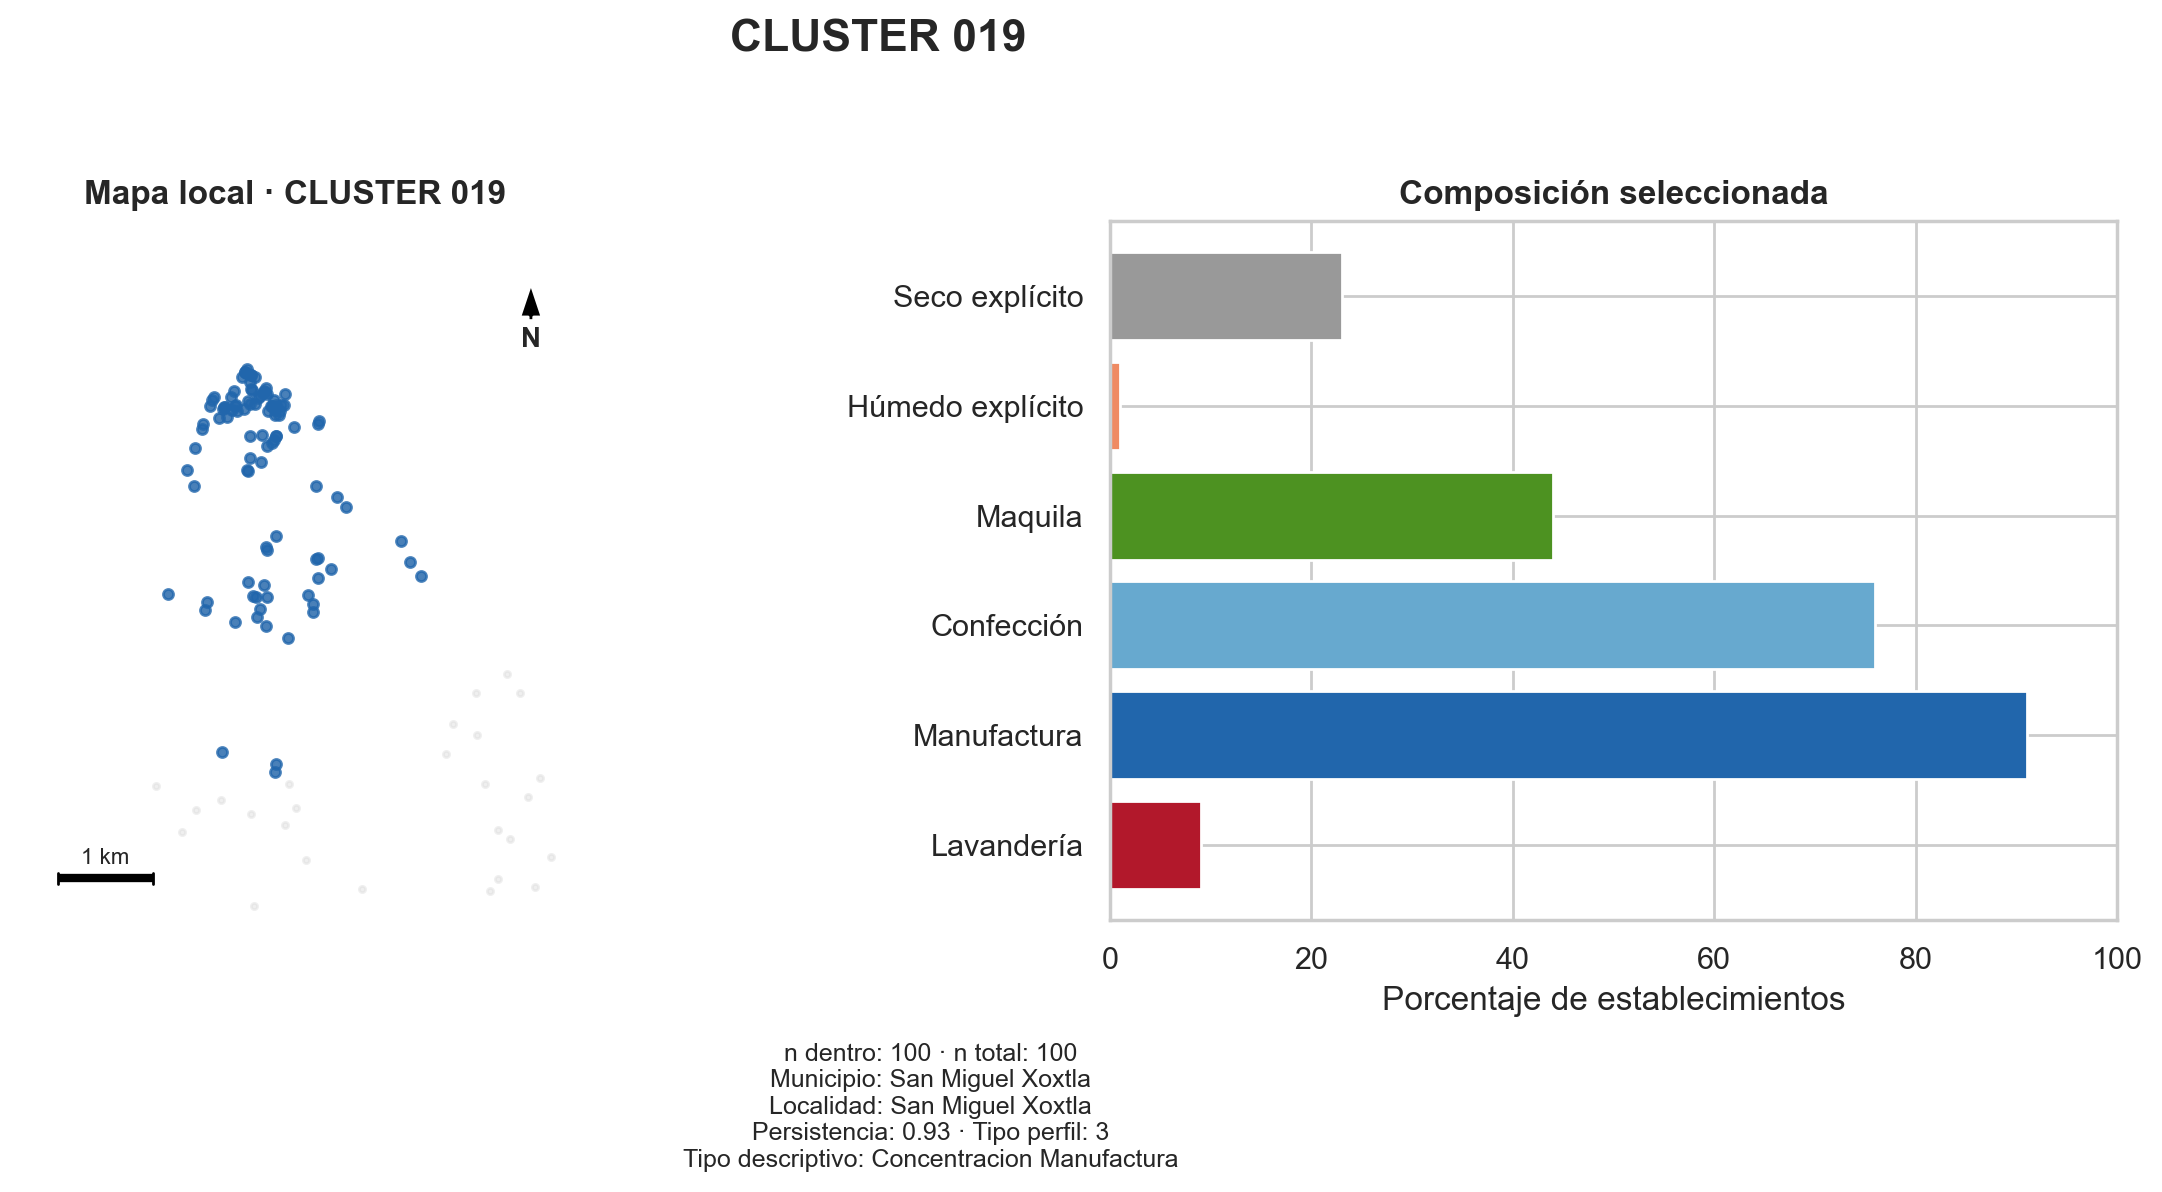
\includegraphics[width=\textwidth]{cluster_019.png}\end{center}
\begin{tabular}{p{0.31\textwidth}p{0.62\textwidth}}
\toprule
Establecimientos & 100 dentro; 0 fuera; 100 total\\
Área convexa & 6.98 km$^2$\\
Persistencia & 0.934\\
Municipio/localidad dominante & San Miguel Xoxtla / San Miguel Xoxtla\\
Lavandería / manufactura & 9.0\% / 91.0\%\\
Confección / maquila & 76.0\% / 44.0\%\\
Húmedo / seco explícito & 1.0\% / 23.0\%\\
Tipología de perfil & 3.0\\
Rasgos distintivos & actividad\_confeccion (lift 1.95) | maquila (lift 3.00) | produccion (lift 2.87) | scian\_textil (lift 1.51) | textil (lift 1.57)\\
Advertencia & Perfil descriptivo multilabel; no prueba relaciones productivas ni ambientales.\\
\bottomrule
\end{tabular}
\clearpage

\section*{Cluster 020}
\addcontentsline{toc}{section}{Cluster 020}
\begin{center}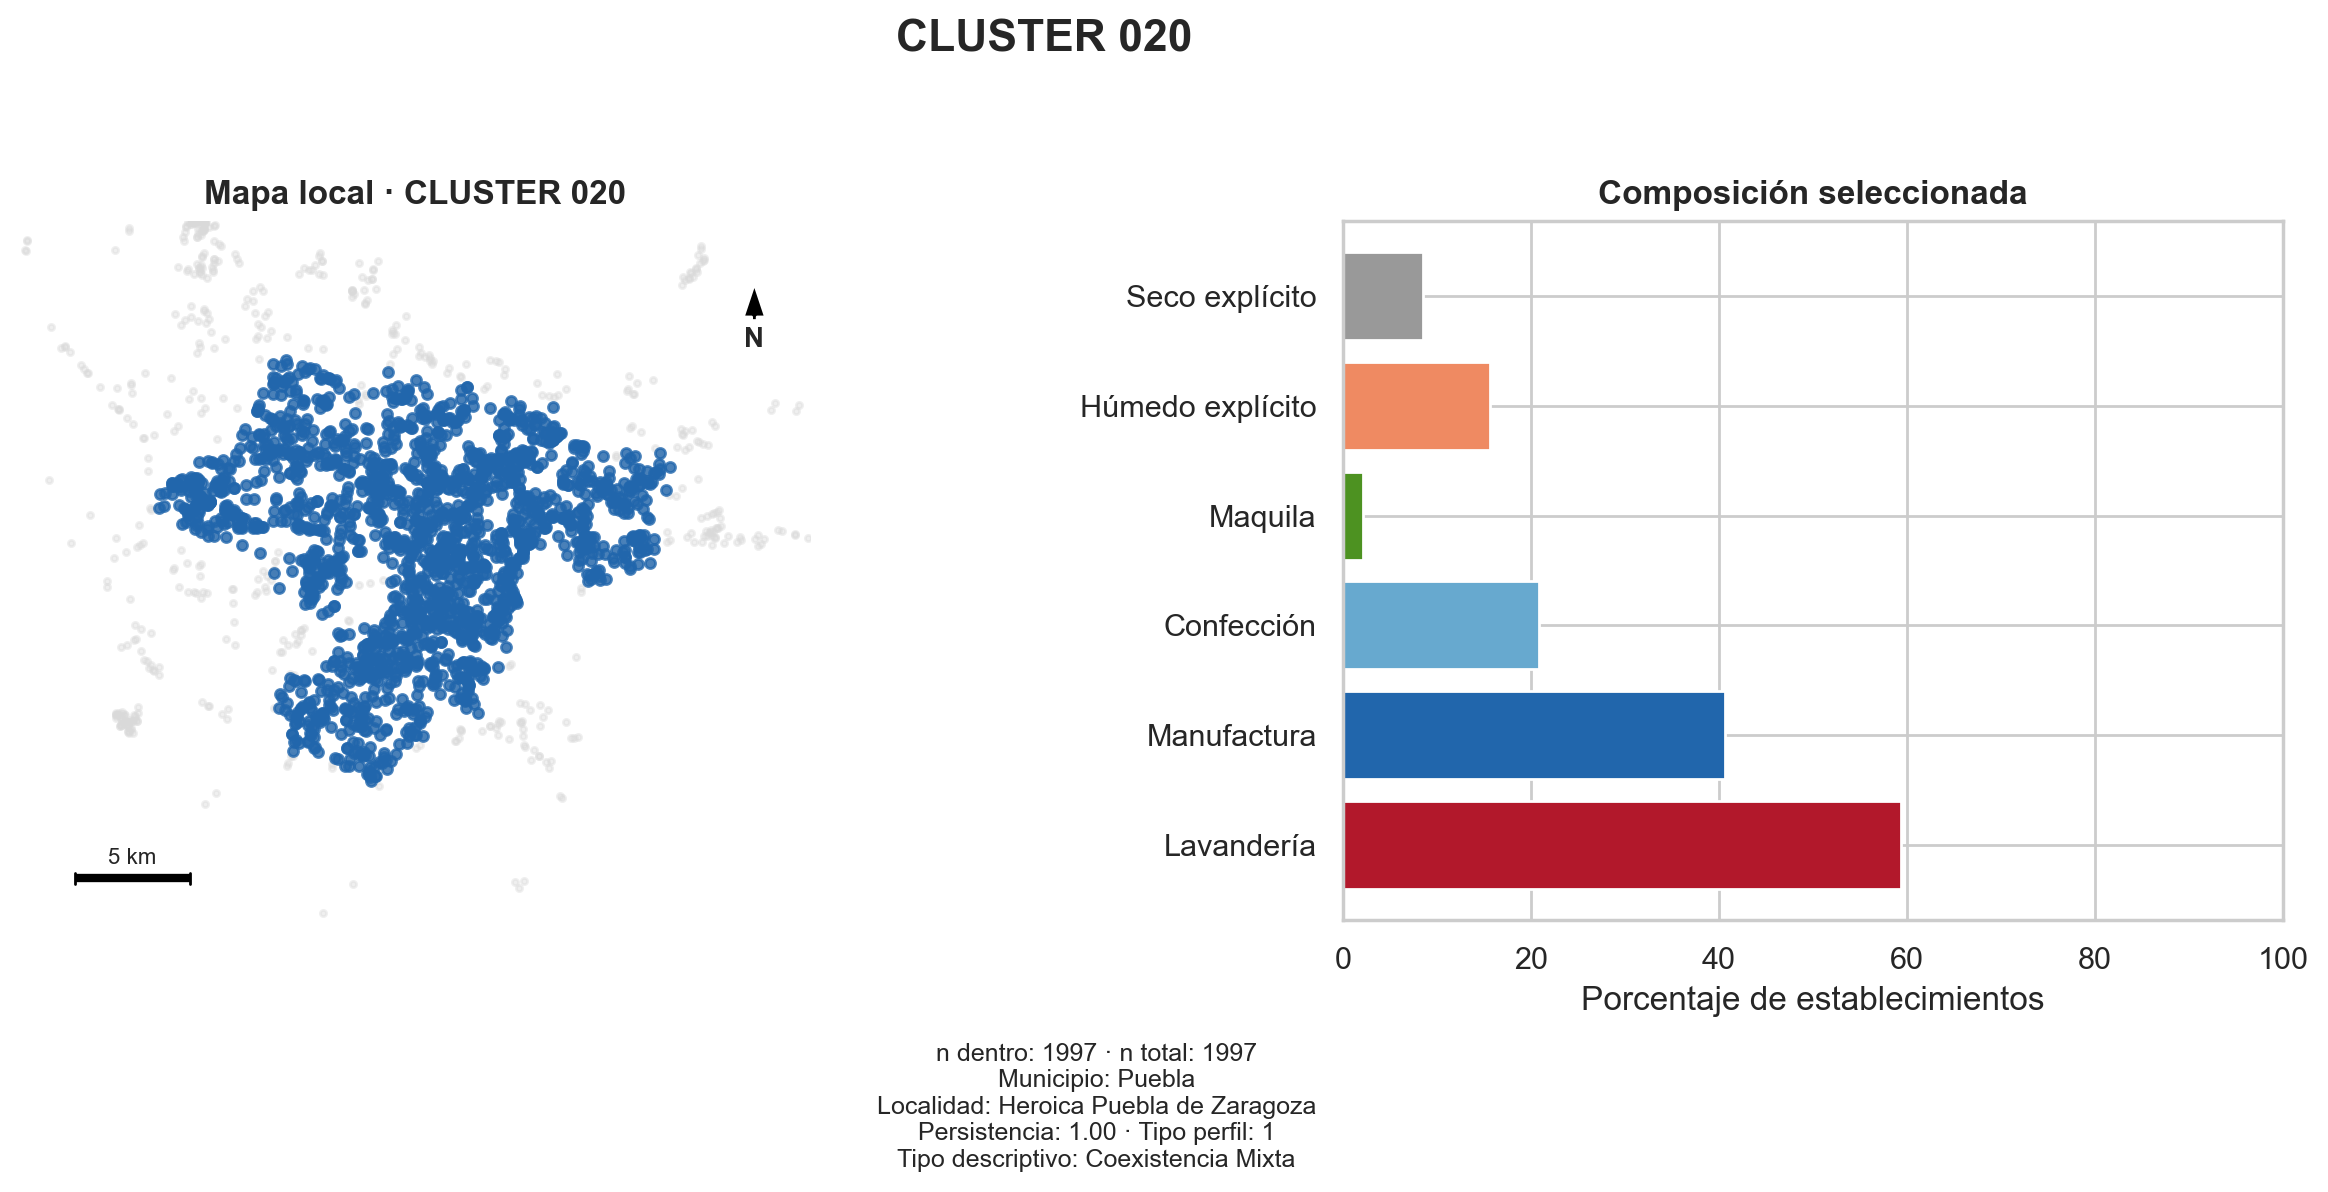
\includegraphics[width=\textwidth]{cluster_020.png}\end{center}
\begin{tabular}{p{0.31\textwidth}p{0.62\textwidth}}
\toprule
Establecimientos & 1997 dentro; 0 fuera; 1997 total\\
Área convexa & 265.29 km$^2$\\
Persistencia & 0.999\\
Municipio/localidad dominante & Puebla / Heroica Puebla de Zaragoza\\
Lavandería / manufactura & 59.3\% / 40.7\%\\
Confección / maquila & 20.9\% / 2.2\%\\
Húmedo / seco explícito & 15.7\% / 8.5\%\\
Tipología de perfil & 1.0\\
Rasgos distintivos & scian\_lavanderia (lift 1.50) | actividad\_lavanderia\_tintoreria (lift 1.50) | lavado\_generico (lift 1.46) | humedo\_explicito (lift 1.70) | actividad\_fabricacion\_telas (lift 1.37)\\
Advertencia & Perfil descriptivo multilabel; no prueba relaciones productivas ni ambientales.\\
\bottomrule
\end{tabular}
\clearpage

\section*{Cluster 021}
\addcontentsline{toc}{section}{Cluster 021}
\begin{center}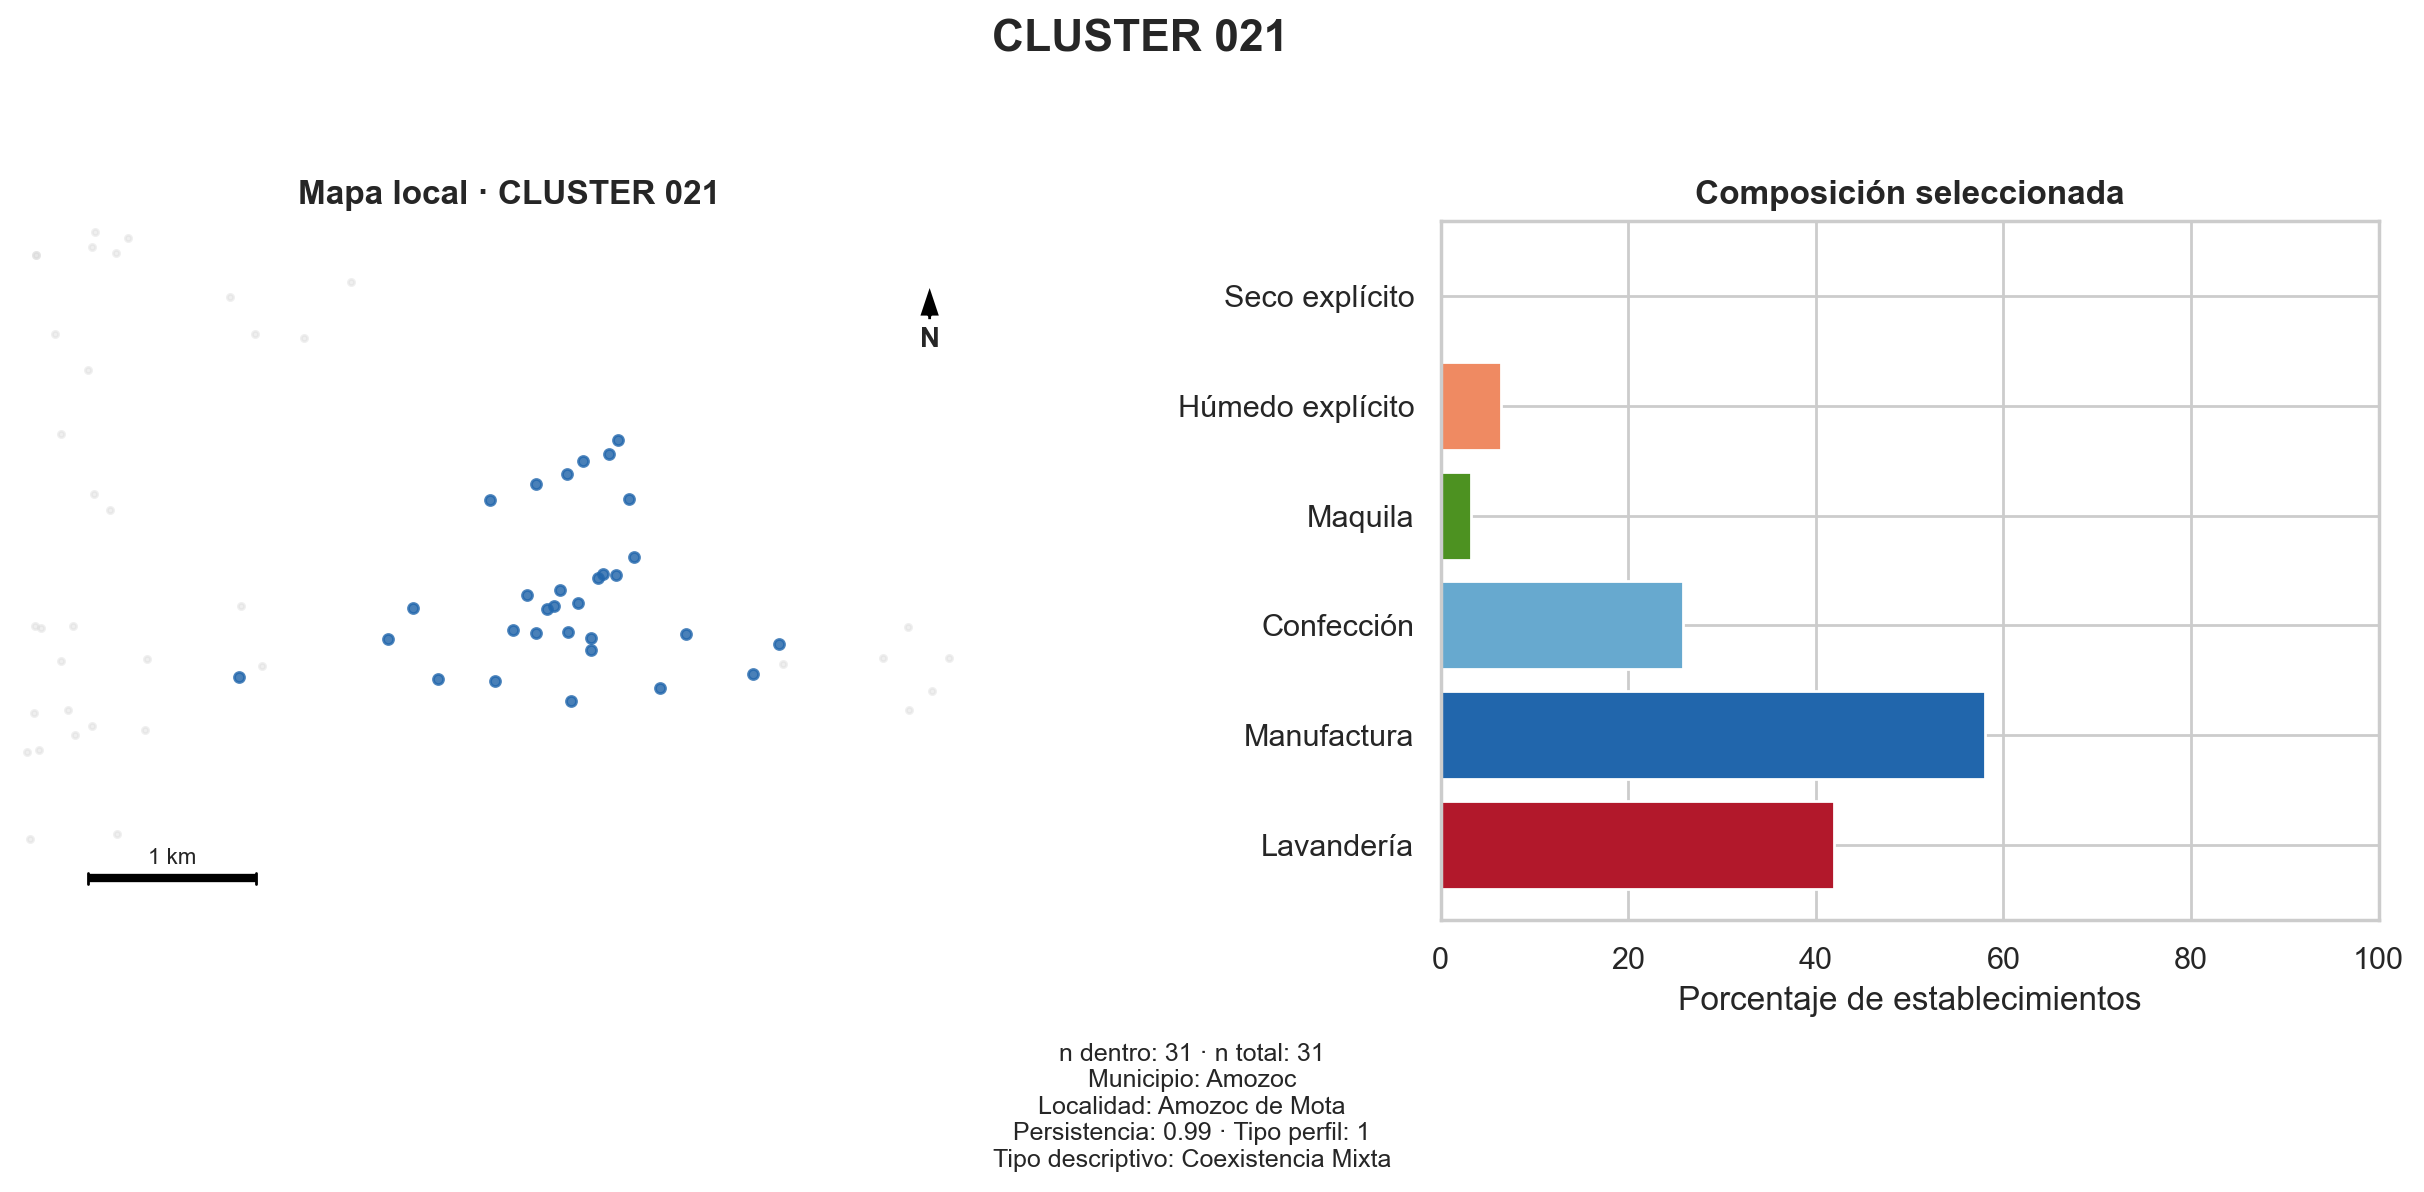
\includegraphics[width=\textwidth]{cluster_021.png}\end{center}
\begin{tabular}{p{0.31\textwidth}p{0.62\textwidth}}
\toprule
Establecimientos & 31 dentro; 0 fuera; 31 total\\
Área convexa & 2.70 km$^2$\\
Persistencia & 0.987\\
Municipio/localidad dominante & Amozoc / Amozoc de Mota\\
Lavandería / manufactura & 41.9\% / 58.1\%\\
Confección / maquila & 25.8\% / 3.2\%\\
Húmedo / seco explícito & 6.5\% / 0.0\%\\
Tipología de perfil & 1.0\\
Rasgos distintivos & Sin rasgos que cumplan todos los umbrales conservadores\\
Advertencia & Perfil descriptivo multilabel; no prueba relaciones productivas ni ambientales.\\
\bottomrule
\end{tabular}
\clearpage

\end{document}